\documentclass[12pt,a4paper]{article}

% -- Packages ------------------------------------------------
\usepackage[margin=2.5cm, headheight=15pt]{geometry}
\usepackage{amsmath, amssymb, amsthm}
\usepackage{graphicx}
\usepackage{booktabs}
\usepackage{array}
\usepackage{listings}
\usepackage{xcolor}
\usepackage{hyperref}
\usepackage{enumitem}
\usepackage{caption}
\usepackage{float}
\usepackage{titlesec}
\usepackage{parskip}
\usepackage{setspace}
\usepackage{fancyhdr}
\usepackage{tcolorbox}
\usepackage{multirow}
\usepackage{longtable}
\usepackage{mdframed}
\usepackage{algorithm}
\usepackage{algpseudocode}

% -- Page style -----------------------------------------------
\pagestyle{fancy}
\fancyhf{}
\rhead{\small N-Body Gravitational Simulation using HPC Techniques}
\lhead{\small High Performance Computing}
\cfoot{\thepage}
\renewcommand{\headrulewidth}{0.4pt}

% -- Spacing --------------------------------------------------
\onehalfspacing

% -- Code listing style ---------------------------------------
\definecolor{codebg}{RGB}{245,245,245}
\definecolor{codeframe}{RGB}{200,200,200}
\definecolor{codecomment}{RGB}{100,100,100}
\definecolor{codekeyword}{RGB}{0,0,180}
\definecolor{codestring}{RGB}{160,0,0}

\lstdefinestyle{cppstyle}{
    language=C++,
    backgroundcolor=\color{codebg},
    frame=single,
    rulecolor=\color{codeframe},
    basicstyle=\ttfamily\small,
    keywordstyle=\color{codekeyword}\bfseries,
    commentstyle=\color{codecomment}\itshape,
    stringstyle=\color{codestring},
    breaklines=true,
    showstringspaces=false,
    tabsize=4,
    numbers=left,
    numberstyle=\tiny\color{gray},
    numbersep=8pt,
    morekeywords={pragma, omp, parallel, for, reduction, schedule,
                  MPI_Init, MPI_Finalize, MPI_Comm_rank, MPI_Comm_size,
                  MPI_Allgatherv, MPI_Allreduce, MPI_Scatterv, MPI_Gatherv,
                  MPI_Bcast, MPI_Wtime, MPI_DOUBLE, MPI_SUM, MPI_COMM_WORLD,
                  MPI_Init_thread, MPI_THREAD_FUNNELED}
}
\lstset{style=cppstyle}

% -- Hyperlink setup ------------------------------------------
\hypersetup{
    colorlinks=true,
    linkcolor=blue!60!black,
    urlcolor=blue!60!black,
    citecolor=blue!60!black
}

% -- Title ----------------------------------------------------
\title{
    \vspace{-1cm}
    {\large Faculty of Engineering --- Computer Engineering Department}\\[0.3em]
    {\large CSE455-High Performance Computing}\\[0.6em]
    \rule{\linewidth}{0.5pt}\\[0.5em]
    {\LARGE \textbf{N-Body Gravitational Simulation}}\\[0.3em]
    {\Large \textbf{using HPC Techniques}}\\[0.3em]
    \rule{\linewidth}{0.5pt}\\[0.6em]
    {\normalsize Sequential, OpenMP, MPI, and Hybrid Parallel Implementations}
}
\author{
    \IfFileExists{uni_logo.png}{%
        
\includegraphics[width=5.6cm]{uni_logo.png}\\[0.9em]
    }{}
    \begin{tabular}{ll}
        Ahmed Ayman Aly        & \texttt{21P0002} \\[3pt]
        Hanna Mohamed Mohamed  & \texttt{21P0162} \\[3pt]
        Marwan NourEldin Farag & \texttt{21P0165} \\[3pt]
        Yehia Mahmoud Lotfy    & \texttt{21P0166} \\[3pt]
        Youssef Ayman Kassab   & \texttt{21P0010} \\
    \end{tabular}
}
\date{May 2026}

% ============================================================
\begin{document}
% ============================================================

\maketitle
\tableofcontents
\clearpage
\listoffigures
\clearpage

% ------------------------------------------------------------
\section{Introduction}
% ------------------------------------------------------------

\subsection{Background and Motivation}

The N-Body problem is one of the oldest and most studied problems in both
classical mechanics and computational science. Originally formulated by Sir
Isaac Newton in the 17th century, it asks: given the initial positions,
velocities, and masses of $N$ bodies, how will they move under mutual
gravitational attraction over time? While the two-body case has a clean
closed-form solution, the three-body and general N-body cases have no
analytical solution and must be solved numerically.

The N-Body problem appears in a wide range of scientific domains:
\begin{itemize}
    \item \textbf{Astrophysics} --- modelling galaxy formation, stellar cluster
          evolution, and planetary system dynamics.
    \item \textbf{Molecular dynamics} --- simulating protein folding and
          molecular interactions in computational chemistry.
    \item \textbf{Plasma physics} --- tracking charged particle interactions
          in fusion research.
    \item \textbf{Computer graphics} --- fluid and particle system simulations
          in real-time rendering.
\end{itemize}

What makes the N-Body problem particularly relevant to High Performance
Computing (HPC) is its inherent computational cost: a direct simulation
requires evaluating every pairwise interaction, leading to
$\mathcal{O}(N^2)$ operations per timestep. For even modest particle counts
(e.g.\ $N = 10{,}000$), a single timestep involves 50 million force
evaluations. Running thousands of timesteps with millions of particles ---
as required in realistic astrophysical simulations --- is only feasible
on modern parallel hardware.

\subsection{Physics of Gravitational Interaction}

\subsubsection*{Newton's Law of Universal Gravitation}

The magnitude of the gravitational force between two point masses $m_i$ and
$m_j$ separated by distance $r$ is:

\begin{equation}
    F = G \frac{m_i \, m_j}{r^2}
\end{equation}

\noindent where $G = 6.674 \times 10^{-11}\,\text{N\,m}^2\,\text{kg}^{-2}$
is the universal gravitational constant. The force is attractive and acts
along the line connecting the two bodies.

In vector form, the force exerted on particle $i$ by particle $j$ is:

\begin{equation}
    \vec{F}_{ij} = G \, m_i \, m_j \,
    \frac{\vec{r}_{ij}}{\left(\left|\vec{r}_{ij}\right|^2 + \epsilon^2\right)^{3/2}}
\end{equation}

\noindent where $\vec{r}_{ij} = \vec{r}_j - \vec{r}_i$ is the displacement
vector from $i$ to $j$. This is the Plummer-softened force law used by the
implementation: the denominator is raised to the power $3/2$, which matches
the code expression \texttt{1.0 / (distSq * sqrt(distSq))}.

\subsubsection*{Softening Factor}

A critical numerical issue arises when two particles pass very close to each
other: the denominator $|\vec{r}_{ij}|^2$ approaches zero, making the force
diverge to infinity. In reality, point masses are an idealisation; real
bodies have finite size. To handle this numerically, a \textbf{softening
parameter} $\epsilon$ is introduced:

\begin{equation}
    \vec{F}_{ij} = G \, m_i \, m_j \,
    \frac{\vec{r}_{ij}}{\left(\left|\vec{r}_{ij}\right|^2 + \epsilon^2\right)^{3/2}}
\end{equation}

This corresponds to Plummer softening in force form, derived from the
softened potential $\phi(r) = -Gm / \sqrt{r^2 + \epsilon^2}$. The force
therefore remains finite at $r=0$. In this project, $\epsilon = 10^{-3}$ is
used. The softened force is indistinguishable from the true force when
$|\vec{r}_{ij}| \gg \epsilon$.

\subsubsection*{Newton's Third Law Optimisation}

By Newton's Third Law, every action has an equal and opposite reaction:

\begin{equation}
    \vec{F}_{ji} = -\vec{F}_{ij}
\end{equation}

This means that for any pair $(i, j)$, computing the force once gives both
$\vec{F}_{ij}$ and $\vec{F}_{ji}$ simultaneously. The naive double-loop
evaluates all $N(N-1)$ ordered pairs. By iterating only over unique
unordered pairs with $j > i$, the number of evaluations drops to:

\begin{equation}
    \frac{N(N-1)}{2}
\end{equation}

This is applied uniformly across all four implementations in this project,
ensuring that speedup comparisons reflect genuine parallelism gains rather
than algorithmic differences.

\subsection{Numerical Integration}

\subsubsection*{Semi-Implicit Euler Method}

The implemented numerical integrator is the \textbf{semi-implicit Euler
method} (also called \textbf{symplectic Euler}). Given the total force
$\vec{F}_i$ on particle $i$ at time $t$, its acceleration is:

\begin{equation}
    \vec{a}_i = \frac{\vec{F}_i}{m_i}
\end{equation}

The velocity is updated first, and the position is then advanced using the
new velocity:

\begin{align}
    \vec{v}_i(t + \Delta t) &= \vec{v}_i(t) + \vec{a}_i(t) \cdot \Delta t \\
    \vec{x}_i(t + \Delta t) &= \vec{x}_i(t) + \vec{v}_i(t + \Delta t) \cdot \Delta t
\end{align}

Like forward Euler, this scheme is first-order accurate: the global error
over $K$ timesteps is $\mathcal{O}(\Delta t)$. However, it is generally more
stable for mechanical systems because it uses the updated velocity in the
position step. It is simple to implement and parallelise, but still
accumulates energy error over long simulations. For the purposes of this
project --- which focuses on parallelism performance rather than long-term
physical accuracy --- the semi-implicit Euler method is sufficient.

\subsubsection*{Computational Cost Per Timestep}

Using Newton's Third Law, the cost breakdown per timestep is:

\begin{center}
\begin{tabular}{llc}
    \toprule
    \textbf{Phase} & \textbf{Operation} & \textbf{Cost} \\
    \midrule
    Force reset     & Zero $N$ accumulators       & $\mathcal{O}(N)$ \\
    Force compute   & $N(N-1)/2$ pair evaluations & $\mathcal{O}(N^2)$ \\
    Integration     & Update $N$ velocities+positions & $\mathcal{O}(N)$ \\
    \midrule
    \textbf{Total}  &                             & $\mathcal{O}(N^2)$ \\
    \bottomrule
\end{tabular}
\end{center}

The force computation phase completely dominates for large $N$, making it
the natural target for parallelisation.

\subsection{Parallel Computing Fundamentals}

\subsubsection*{Speedup and Amdahl's Law}

Speedup $S$ measures how much faster a parallel program runs compared to
the sequential baseline using $W$ workers:

\begin{equation}
    S(W) = \frac{T_1}{T_W}
\end{equation}

\noindent where $T_1$ is the sequential time and $T_W$ is the parallel time
with $W$ workers. Amdahl's Law sets a theoretical upper bound: if fraction
$f$ of the program is parallelisable and fraction $(1-f)$ is inherently
serial, then:

\begin{equation}
    S(W) \leq \frac{1}{(1-f) + \frac{f}{W}}
\end{equation}

As $W \to \infty$, $S \to 1/(1-f)$. This means even a 5\% serial fraction
caps the maximum speedup at $20\times$ regardless of hardware.

\subsubsection*{Parallel Efficiency}

Parallel efficiency $E$ measures how well each worker is utilised:

\begin{equation}
    E(W) = \frac{S(W)}{W} = \frac{T_1}{W \cdot T_W}
\end{equation}

An efficiency of 1.0 (100\%) means all workers are busy doing useful work
with zero overhead. In practice, synchronisation, communication, and load
imbalance all reduce efficiency below 1.

\subsubsection*{Shared vs.\ Distributed Memory}

Two fundamentally different parallel architectures are used in this project:

\begin{itemize}
    \item \textbf{Shared memory (OpenMP):} All threads run in the same process
          and access the same RAM directly. Communication is free (a simple
          read/write), but threads must synchronise to avoid race conditions.
          Scales to the number of cores on one physical machine.

    \item \textbf{Distributed memory (MPI):} Each process has its own private
          memory. Communication requires explicit message passing
          (\texttt{MPI\_Send}/\texttt{MPI\_Recv} or collective operations).
          Can scale across thousands of nodes, but every data exchange has a
          latency and bandwidth cost.
\end{itemize}

The \textbf{Hybrid model} combines both: MPI distributes work across nodes,
OpenMP parallelises within each node. This is the standard approach on
modern HPC clusters (e.g.\ Summit, Frontier) where each node has many cores
sharing local RAM, and nodes are connected via a high-speed network.

\subsection{Objectives}

This project aims to:

\begin{enumerate}
    \item Implement a correct 2D N-Body gravitational simulation in four
          parallel programming models: Sequential, OpenMP, MPI, and Hybrid
          (MPI + OpenMP).
    \item Apply Newton's Third Law optimisation uniformly across all versions
          to ensure fair performance comparisons.
    \item Measure wall-clock time, speedup, and parallel efficiency across
          particle counts $N \in \{100, 500, 1000, 2000, 5000\}$.
    \item Analyse the impact of communication overhead (MPI), thread
          synchronisation (OpenMP), and load imbalance (triangular loop)
          on scalability.
    \item Identify the crossover points where parallelism becomes beneficial
          and explain the observed behaviour using HPC theory.
    \item Discuss the advantages of the Hybrid model for multi-node cluster
          deployments compared to single-node execution.
\end{enumerate}

% ------------------------------------------------------------
\section{Implementation Details}
% ------------------------------------------------------------

\subsection{Project Structure}

\begin{center}
\begin{tabular}{ll}
    \toprule
    \textbf{File} & \textbf{Purpose} \\
    \midrule
    \texttt{common.h}      & Shared data structures, initialisation, CSV output \\
    \texttt{sequential.cpp} & Single-threaded baseline \\
    \texttt{openmp.cpp}    & Shared-memory parallelism (OpenMP) \\
    \texttt{mpi.cpp}       & Distributed-memory parallelism (MPI) \\
    \texttt{hybrid.cpp}    & Two-level parallelism (MPI + OpenMP) \\
    \texttt{benchmark.ps1} & Automated benchmark script \\
    \texttt{Makefile}      & Build system \\
    \bottomrule
\end{tabular}
\end{center}

\subsection{Data Structures}

All versions share structures defined in \texttt{common.h}.

\subsubsection*{Particle (Array of Structures)}

\begin{lstlisting}
struct Particle {
    double x, y;    // Position
    double vx, vy;  // Velocity
    double mass;    // Mass
};
\end{lstlisting}

Used by the sequential and OpenMP versions for cache-friendly sequential access.

\subsubsection*{Flat Separate Arrays (Structure of Arrays)}

The MPI and Hybrid versions decompose particle data into separate flat arrays
(\texttt{all\_x[]}, \texttt{all\_y[]}, \texttt{all\_vx[]}, \texttt{all\_vy[]},
\texttt{all\_mass[]}) to make MPI collectives straightforward ---
\texttt{MPI\_Scatterv}, \texttt{MPI\_Allgatherv}, and \texttt{MPI\_Allreduce}
all require contiguous buffers of a single type.

\subsubsection*{Simulation Parameters}

\begin{lstlisting}
struct SimParams {
    int    N;           // Number of particles
    double dt;          // Time step
    int    iterations;  // Number of simulation steps
    int    output_freq; // CSV output frequency (0 = disabled)
};
\end{lstlisting}

Configured entirely via command-line arguments for reproducible experiments.

\subsubsection*{Initialisation}

All four versions use the same \texttt{initParticles()} function with a
\textbf{fixed random seed (42)}:
\begin{itemize}
    \item Positions uniformly in $[0,\,1000]$
    \item Velocities uniformly in $[-1,\,1]$
    \item Masses uniformly in $[10^{10},\,10^{12}]$
\end{itemize}

This guarantees identical initial conditions and directly comparable results
across all four implementations.

% ------------------------------------
\subsection{Sequential Version}

The sequential version serves as the algorithmic and performance baseline.
It implements the complete simulation loop without any parallelism, so that
all measured speedups are relative to a well-optimised single-threaded run.

\subsubsection*{Algorithm}

\begin{algorithm}[H]
\caption{Sequential N-Body Simulation}
\begin{algorithmic}[1]
\State Initialise $N$ particles (positions, velocities, masses)
\For{$\textit{iter} = 1$ \textbf{to} $\textit{iterations}$}
    \State Reset force accumulators: $f_x[i] \leftarrow 0,\; f_y[i] \leftarrow 0 \quad \forall i$
    \For{$i = 0$ \textbf{to} $N-2$}
        \For{$j = i+1$ \textbf{to} $N-1$}
            \State Compute $\vec{F}_{ij}$ using softened gravity
            \State $f_x[i] \mathrel{+}= F_x$;\quad $f_y[i] \mathrel{+}= F_y$
            \State $f_x[j] \mathrel{-}= F_x$;\quad $f_y[j] \mathrel{-}= F_y$ \Comment{Newton's 3rd law}
        \EndFor
    \EndFor
    \For{$i = 0$ \textbf{to} $N-1$}
        \State $a_x \leftarrow f_x[i] / m_i$;\quad $a_y \leftarrow f_y[i] / m_i$
        \State $v_x[i] \mathrel{+}= a_x \cdot \Delta t$;\quad $v_y[i] \mathrel{+}= a_y \cdot \Delta t$
        \State $x[i] \mathrel{+}= v_x[i] \cdot \Delta t$;\quad $y[i] \mathrel{+}= v_y[i] \cdot \Delta t$
    \EndFor
\EndFor
\end{algorithmic}
\end{algorithm}

\subsubsection*{Force Computation}

\begin{lstlisting}
for (int i = 0; i < N - 1; i++) {
    for (int j = i + 1; j < N; j++) {
        double dx = particles[j].x - particles[i].x;
        double dy = particles[j].y - particles[i].y;
        // Softened squared distance to prevent singularity
        double distSq   = dx*dx + dy*dy + SOFTENING*SOFTENING;
        double invDist3 = 1.0 / (distSq * std::sqrt(distSq));
        double F        = G * particles[i].mass * particles[j].mass * invDist3;
        fx[i] += F * dx;   fy[i] += F * dy;
        fx[j] -= F * dx;   fy[j] -= F * dy;  // equal and opposite
    }
}
\end{lstlisting}

The inner computation for each pair involves: 2 subtractions, 5 multiplications,
2 additions (distance), 1 square root, 1 division, and 8 accumulations ---
approximately 20 floating-point operations per pair. At $N=5000$ this is
roughly $\frac{5000 \times 4999}{2} \approx 12.5 \times 10^6$ pairs
$\times$ 20 FLOP $= 250 \times 10^6$ FLOP per timestep.

\subsubsection*{Semi-Implicit Euler Integration}

\begin{lstlisting}
for (int i = 0; i < N; i++) {
    double ax = fx[i] / particles[i].mass;
    double ay = fy[i] / particles[i].mass;
    particles[i].vx += ax * dt;
    particles[i].vy += ay * dt;
    particles[i].x  += particles[i].vx * dt;
    particles[i].y  += particles[i].vy * dt;
}
\end{lstlisting}

\subsubsection*{Output}

At the end of each simulation, the program reports:
\begin{itemize}
    \item Total wall-clock time (via \texttt{std::chrono::high\_resolution\_clock})
    \item Pairs per second: $\frac{N(N-1)}{2} \times \textit{iterations} / T$
    \item Optionally writes per-step particle states to a CSV file
          (\texttt{output\_sequential.csv}) when \texttt{output\_freq > 0}
\end{itemize}

% ------------------------------------
\subsection{OpenMP Version}

The OpenMP version targets the force computation loop -- the dominant
$\mathcal{O}(N^2)$ phase. It runs within a single process but distributes
the outer loop iterations across multiple threads that share the same
address space.

\subsubsection*{Race Condition Problem}

Newton's Third Law requires writing to both \texttt{fx[i]} and \texttt{fx[j]}
inside the same iteration. When two threads handle overlapping $i$-values, they
may simultaneously try to update the same \texttt{fx[j]} element:

\begin{center}
\begin{tabular}{ll}
    \toprule
    \textbf{Thread 0} & \textbf{Thread 1} \\
    \midrule
    Computes pair $(0, 5)$: writes \texttt{fx[5]} & \\
    & Computes pair $(3, 5)$: writes \texttt{fx[5]} \\
    \multicolumn{2}{c}{$\Rightarrow$ One update is lost (data race)} \\
    \bottomrule
\end{tabular}
\end{center}

This is a classic \textbf{write-after-write} race condition. Using
\texttt{atomic} operations would work but would serialize every write to
shared elements. OpenMP \textbf{array reduction} is the optimal solution.

\subsubsection*{Array Reduction Mechanism}

Each thread gets a \emph{private} copy of the full \texttt{fx[]} and
\texttt{fy[]} arrays initialised to zero. Threads write to their own
copies independently (no synchronisation needed). At the parallel region
barrier, OpenMP sums all private copies element-by-element into the
shared result:

\begin{equation}
    \texttt{fx}[i]_{\text{final}} = \sum_{t=0}^{T-1} \texttt{fx}[i]_{\text{thread } t}
\end{equation}

This merge costs $\mathcal{O}(N \times T)$ time at the barrier, which is
negligible compared to the $\mathcal{O}(N^2)$ computation.

\subsubsection*{Parallel Force Loop}

\begin{lstlisting}
// Raw arrays required for OpenMP array reduction syntax
double* fx = new double[N];
double* fy = new double[N];

#pragma omp parallel for schedule(dynamic, 16) \
        reduction(+: fx[0:N], fy[0:N])
for (int i = 0; i < N - 1; i++) {
    for (int j = i + 1; j < N; j++) {
        double dx = particles[j].x - particles[i].x;
        double dy = particles[j].y - particles[i].y;
        double distSq   = dx*dx + dy*dy + SOFTENING*SOFTENING;
        double invDist3 = 1.0 / (distSq * std::sqrt(distSq));
        double F   = G * particles[i].mass * particles[j].mass * invDist3;
        double f_x = F * dx;
        double f_y = F * dy;
        fx[i] += f_x;   fy[i] += f_y;
        fx[j] -= f_x;   fy[j] -= f_y;   // Newton's 3rd law
    }
}
\end{lstlisting}

\subsubsection*{Scheduling Strategy}

The triangular loop structure creates an inherent load imbalance:
iteration $i=0$ processes $N-1$ pairs, while iteration $i=N-2$ processes
only 1 pair. With static scheduling, the first thread would receive
disproportionately more work. \texttt{schedule(dynamic, 16)} assigns chunks
of 16 consecutive $i$-values at runtime as threads become free, keeping all
threads utilised throughout:

\begin{center}
\begin{tabular}{lcc}
    \toprule
    \textbf{Schedule} & \textbf{Idle time} & \textbf{Overhead} \\
    \midrule
    \texttt{static}          & High (uneven work) & Very low \\
    \texttt{dynamic, 1}      & Near zero          & High (per-iteration queue) \\
    \texttt{dynamic, 16}     & Very low           & Low (chunk amortises cost) \\
    \bottomrule
\end{tabular}
\end{center}

A chunk size of 16 was chosen as a balance: small enough to distribute
the uneven tail of the loop, large enough to amortise the runtime
scheduling overhead.

% ------------------------------------
\subsection{MPI Version}

\subsubsection*{Particle Distribution}

The $N$ particles are divided among $P$ MPI processes using a \textbf{block
partition}. Process $r$ owns particles in the index range
$[\textit{displs}[r],\;\textit{displs}[r] + \textit{counts}[r])$.
Any remainder $N \bmod P$ is distributed one extra particle to the
first $N \bmod P$ ranks:

\begin{equation}
    \textit{counts}[r] = \left\lfloor \frac{N}{P} \right\rfloor +
    \begin{cases} 1 & \text{if } r < N \bmod P \\ 0 & \text{otherwise} \end{cases}
\end{equation}

\subsubsection*{Data Layout}

Unlike the sequential and OpenMP versions which use an Array-of-Structures
layout (\texttt{Particle} struct), the MPI version uses a Structure-of-Arrays
layout with separate flat buffers for each field. This is required because MPI
collectives operate on contiguous arrays of a single datatype:

\begin{lstlisting}
std::vector<double> all_x(N), all_y(N);       // global positions
std::vector<double> all_vx(N), all_vy(N);     // global velocities
std::vector<double> all_mass(N);               // global masses (constant)

std::vector<double> local_x(local_n), local_y(local_n);
std::vector<double> local_vx(local_n), local_vy(local_n);
\end{lstlisting}

\subsubsection*{Initialisation and Data Scatter}

Rank 0 initialises all particles using the same \texttt{initParticles()}
function (same seed). Masses are broadcast once with \texttt{MPI\_Bcast}
(they never change). Positions and velocities are scattered to each rank:

\begin{lstlisting}
MPI_Bcast(all_mass.data(), N, MPI_DOUBLE, 0, MPI_COMM_WORLD);
MPI_Scatterv(all_x.data(),  counts.data(), displs.data(), MPI_DOUBLE,
             local_x.data(), local_n, MPI_DOUBLE, 0, MPI_COMM_WORLD);
// repeated for y, vx, vy
\end{lstlisting}

\subsubsection*{Per-Timestep Algorithm}

\begin{algorithm}[H]
\caption{MPI N-Body Timestep (Newton's 3rd Law + Allreduce)}
\begin{algorithmic}[1]
\State \textbf{MPI\_Allgatherv}$(local\_x, local\_y) \to (all\_x, all\_y)$
\State Reset partial force arrays: $\textit{partial\_fx}[k] \leftarrow 0 \quad \forall k \in [0,N)$
\For{$i = 0$ \textbf{to} $\textit{local\_n}-1$} \Comment{local particles only}
    \State $\textit{global\_i} \leftarrow \textit{local\_start} + i$
    \For{$j = \textit{global\_i}+1$ \textbf{to} $N-1$}
        \State Compute $\vec{F}_{ij}$
        \State $\textit{partial\_fx}[\textit{global\_i}] \mathrel{+}= F_x$
        \State $\textit{partial\_fx}[j] \mathrel{-}= F_x$ \Comment{write to remote slot}
    \EndFor
\EndFor
\State \textbf{MPI\_Allreduce}$(\textit{partial\_fx}, \textit{total\_fx}, N, \text{MPI\_SUM})$
\State \textbf{MPI\_Allreduce}$(\textit{partial\_fy}, \textit{total\_fy}, N, \text{MPI\_SUM})$
\For{$i = 0$ \textbf{to} $\textit{local\_n}-1$}
    \State Update local velocity and position using $\textit{total\_fx}[\textit{global\_i}]$
\EndFor
\end{algorithmic}
\end{algorithm}

\subsubsection*{Why MPI\_Allreduce for Forces?}

When process $r$ computes pair $(\textit{global\_i}, j)$ and $j$ belongs to
process $r'$, the force $-\vec{F}$ must be applied to particle $j$. Since
processes cannot write into each other's memory directly, each process
accumulates its contributions for all $N$ particles into a local
\texttt{partial\_fx[]} array. \texttt{MPI\_Allreduce(MPI\_SUM)} then sums
all these partial arrays element-by-element across every process, giving
every rank the correct total force for all particles:

\begin{lstlisting}
MPI_Allreduce(partial_fx.data(), total_fx.data(), N,
              MPI_DOUBLE, MPI_SUM, MPI_COMM_WORLD);
MPI_Allreduce(partial_fy.data(), total_fy.data(), N,
              MPI_DOUBLE, MPI_SUM, MPI_COMM_WORLD);
\end{lstlisting}

Each process then reads only \texttt{total\_fx[local\_start .. local\_start+local\_n-1]}
to update its own particles.

% ------------------------------------
\subsection{Hybrid (MPI + OpenMP) Version}

The Hybrid version stacks both levels of parallelism: MPI manages
inter-process distribution, while OpenMP threads handle the force computation
within each process.

\subsubsection*{Thread Safety Requirement}

MPI and OpenMP must be used carefully together. MPI has four thread safety
levels:

\begin{center}
\begin{tabular}{ll}
    \toprule
    \textbf{Level} & \textbf{Meaning} \\
    \midrule
    \texttt{MPI\_THREAD\_SINGLE}    & Only one thread will execute \\
    \texttt{MPI\_THREAD\_FUNNELED}  & Only master thread calls MPI \\
    \texttt{MPI\_THREAD\_SERIALIZED}& One thread at a time calls MPI \\
    \texttt{MPI\_THREAD\_MULTIPLE}  & Any thread can call MPI \\
    \bottomrule
\end{tabular}
\end{center}

This implementation uses \texttt{MPI\_THREAD\_FUNNELED}: only the master
thread (thread 0) ever calls MPI functions. All \texttt{MPI\_Allgatherv}
and \texttt{MPI\_Allreduce} calls are made outside the
\texttt{\#pragma omp parallel} region, ensuring correctness without
requiring full \texttt{MPI\_THREAD\_MULTIPLE} support.

\subsubsection*{Initialisation}

\begin{lstlisting}
int provided;
MPI_Init_thread(&argc, &argv, MPI_THREAD_FUNNELED, &provided);
\end{lstlisting}

\subsubsection*{Two-Level Force Loop}

\begin{lstlisting}
// partial_fx/fy are raw C arrays (required for OMP array reduction)
double* partial_fx = new double[N];
double* partial_fy = new double[N];

// Reset (serial -- outside parallel region)
for (int k = 0; k < N; k++) partial_fx[k] = partial_fy[k] = 0.0;

// OMP threads divide the local particle range; array reduction
// handles intra-process race conditions on partial_fx[j]
#pragma omp parallel for schedule(dynamic, 16) \
        reduction(+: partial_fx[0:N], partial_fy[0:N])
for (int i = 0; i < local_n; i++) {
    int global_i = local_start + i;
    for (int j = global_i + 1; j < N; j++) {
        double dx = all_x[j] - local_x[i];
        double dy = all_y[j] - local_y[i];
        double distSq   = dx*dx + dy*dy + SOFTENING*SOFTENING;
        double invDist3 = 1.0 / (distSq * std::sqrt(distSq));
        double F   = G * all_mass[global_i] * all_mass[j] * invDist3;
        double f_x = F * dx;
        double f_y = F * dy;
        partial_fx[global_i] += f_x;
        partial_fy[global_i] += f_y;
        partial_fx[j]        -= f_x;   // Newton's 3rd law
        partial_fy[j]        -= f_y;
    }
}
// Master thread proceeds here; OMP barrier guarantees all writes done
MPI_Allreduce(partial_fx, total_fx.data(), N, MPI_DOUBLE, MPI_SUM, MPI_COMM_WORLD);
MPI_Allreduce(partial_fy, total_fy.data(), N, MPI_DOUBLE, MPI_SUM, MPI_COMM_WORLD);
\end{lstlisting}

\subsubsection*{Work Decomposition Summary}

\begin{center}
\begin{tabular}{lll}
    \toprule
    \textbf{Level} & \textbf{Partitions} & \textbf{Mechanism} \\
    \midrule
    MPI  & $N$ particles into $P$ blocks  & \texttt{MPI\_Scatterv} / block partition \\
    OMP  & $\textit{local\_n}$ iterations into $T$ chunks & \texttt{schedule(dynamic, 16)} \\
    Both & Force accumulation             & OMP array reduction + \texttt{MPI\_Allreduce} \\
    \bottomrule
\end{tabular}
\end{center}

For $P$ MPI processes and $T$ OpenMP threads per process, the total worker
count is $W = P \times T$. The Hybrid model is most efficient when $P$ is
kept small (minimising MPI collective overhead) and $T$ is maximised to
use all available cores per node via shared memory.

% ------------------------------------------------------------
\section{Results}
% ------------------------------------------------------------

\subsection{Experimental Setup}

All experiments were run on a single machine under identical conditions.
The benchmark script (\texttt{benchmark.ps1}) compiled all four executables
with the same flags and ran each configuration three times, reporting the
single run result per configuration (variation was less than 2\% across
runs for $N \geq 500$).

\begin{center}
\begin{tabular}{ll}
    \toprule
    \textbf{Parameter} & \textbf{Value} \\
    \midrule
    Machine          & \textit{TODO: CPU model, core count, RAM} \\
    OS               & Windows \\
    Compiler         & G++ \texttt{-O2 -std=c++17} \\
    MPI              & Microsoft MPI (MS-MPI) \\
    OpenMP           & GCC built-in \\
    Particle counts  & 100, 500, 1000, 2000, 5000 \\
    Time step $dt$   & 0.01 \\
    Iterations       & 100 ($N \leq 500$),\; 50 ($N=1000$),\; 30 ($N=2000$),\;
                       15 ($N=5000$) \\
    OMP thread counts & 2, 4, 8 \\
    MPI process counts & 2, 4 \\
    Hybrid combos    & $2P{\times}2T$,\; $2P{\times}4T$,\; $4P{\times}2T$ \\
    \bottomrule
\end{tabular}
\end{center}

The iteration count is scaled down for larger $N$ to keep each configuration's
wall time below approximately 2 seconds, enabling a complete benchmark sweep
across all configurations in reasonable time. Speedup and efficiency values
remain valid because they are normalised per-$N$: the sequential baseline
at each $N$ uses the same iteration count as the parallel versions.

Speedup and parallel efficiency are defined as:

\begin{equation}
    S = \frac{T_{\text{sequential}}}{T_{\text{parallel}}}
    \qquad\qquad
    E = \frac{S}{W}
\end{equation}

where $W = P \times T$ is the total worker count (MPI processes times OpenMP
threads per process).

\subsection{Wall-Clock Time}

Table~\ref{tab:walltime} reports the total wall-clock time in seconds for
each configuration. Times include the simulation loop only (excluding
initialisation and final output). For the sequential version, timing uses
\texttt{std::chrono::high\_resolution\_clock}. For MPI and Hybrid versions,
\texttt{MPI\_Wtime()} is used on rank 0.

\begin{table}[H]
\centering
\caption{Wall-clock time (seconds) for all configurations and particle counts.}
\label{tab:walltime}
\begin{tabular}{rcccccccc}
    \toprule
    $N$ & Seq & OMP 2T & OMP 4T & OMP 8T & MPI 2P & MPI 4P
        & Hyb $2{\times}4$ & Hyb $4{\times}2$ \\
    \midrule
    100  & 0.00244 & 0.00838 & 0.01030 & 0.01539
         & 0.00364 & 0.00223 & 0.00783 & 0.00850 \\
    500  & 0.06984 & 0.04226 & 0.02676 & 0.02571
         & 0.05007 & 0.03828 & 0.02321 & 0.02386 \\
    1000 & 0.12652 & 0.06694 & 0.04270 & 0.02878
         & 0.09638 & 0.05685 & 0.03493 & 0.03854 \\
    2000 & 0.30091 & 0.15403 & 0.08479 & 0.05425
         & 0.22965 & 0.13782 & 0.06427 & 0.07743 \\
    5000 & 0.93055 & 0.46782 & 0.24528 & 0.13532
         & 0.69949 & 0.41418 & 0.18797 & 0.23890 \\
    \bottomrule
\end{tabular}
\end{table}

\noindent\textbf{Key observations from raw timing:}
\begin{itemize}
    \item At $N=100$, the sequential run completes in under 3\,ms ---
          all parallel configurations are \emph{slower} due to startup
          and communication overhead.
    \item OpenMP 8T is the fastest configuration at every $N \geq 500$.
    \item MPI 4P is consistently slower than OpenMP 4T despite having the
          same number of workers, reflecting communication overhead.
    \item At $N=5000$, Hybrid $2P \times 4T$ achieves 0.188\,s ---
          competitive with but not exceeding OpenMP 8T at 0.135\,s.
\end{itemize}

\subsection{Speedup Analysis}

Table~\ref{tab:speedup} shows speedup relative to the sequential baseline
at each particle count.

\begin{table}[H]
\centering
\caption{Speedup $S = T_{\text{seq}} / T_{\text{parallel}}$.
         Values $<1$ indicate the parallel version is slower than sequential.}
\label{tab:speedup}
\begin{tabular}{rccccccc}
    \toprule
    $N$ & OMP 2T & OMP 4T & OMP 8T & MPI 2P & MPI 4P
        & Hyb $2{\times}4$ & Hyb $4{\times}2$ \\
    \midrule
    100  & 0.29 & 0.24 & 0.16 & 0.67 & 1.09 & 0.31 & 0.29 \\
    500  & 1.65 & 2.61 & 2.72 & 1.39 & 1.82 & 3.01 & 2.93 \\
    1000 & 1.89 & 2.96 & 4.40 & 1.31 & 2.23 & 3.62 & 3.28 \\
    2000 & 1.95 & 3.55 & 5.55 & 1.31 & 2.18 & 4.68 & 3.89 \\
    5000 & 1.99 & 3.79 & \textbf{6.88} & 1.33 & 2.25
         & \textbf{4.95} & 3.90 \\
    \bottomrule
\end{tabular}
\end{table}

\noindent\textbf{Key observations:}
\begin{itemize}
    \item \textbf{OpenMP scales best} and improves consistently with $N$.
          At $N=5000$, 8 threads delivers $6.88\times$ --- the highest
          speedup of any single configuration tested.
    \item \textbf{MPI speedup plateaus} at approximately $1.33\times$ (2P)
          and $2.25\times$ (4P) regardless of $N$, reflecting the constant
          communication cost per timestep.
    \item \textbf{Hybrid $2P \times 4T$ outperforms Hybrid $4P \times 2T$}
          at every $N$, confirming that minimising MPI processes is
          preferable on a single node.
    \item At \textbf{$N=100$, MPI 4P is the only configuration to achieve
          speedup $>1$} (1.09$\times$) --- all others are slower than
          sequential.
\end{itemize}

\subsection{Parallel Efficiency}

Table~\ref{tab:efficiency} shows efficiency $E = S/W$ for each configuration.
An efficiency of 1.0 represents ideal linear scaling.

\begin{table}[H]
\centering
\caption{Parallel efficiency $E = S/W$ (\%). Hybrid columns use $W=8$ workers.
         Values above 80\% are highlighted in \textbf{bold}.}
\label{tab:efficiency}
\begin{tabular}{rccccccc}
    \toprule
    $N$ & OMP 2T & OMP 4T & OMP 8T & MPI 2P & MPI 4P
        & Hyb $2{\times}4$ & Hyb $4{\times}2$ \\
    \midrule
    100  & 14.6 & 5.9  & 2.0  & 33.5 & 27.4 &  3.9 &  3.6 \\
    500  & 82.6 & 65.2 & 33.9 & 69.7 & 45.6 & 37.6 & 36.6 \\
    1000 & \textbf{94.5} & 74.1 & 54.9 & 65.6 & 55.6 & 45.3 & 41.0 \\
    2000 & \textbf{97.7} & \textbf{88.7} & 69.3 & 65.5 & 54.6 & 58.5 & 48.6 \\
    5000 & \textbf{99.5} & \textbf{94.8} & \textbf{86.0}
         & 66.5 & 56.2 & 61.9 & 48.7 \\
    \bottomrule
\end{tabular}
\end{table}

\noindent\textbf{Key observations:}
\begin{itemize}
    \item \textbf{OpenMP 2T reaches 99.5\% efficiency at $N=5000$} ---
          essentially perfect linear scaling. This is because the
          parallelisable fraction $f \approx 1.0$ for large $N$, and the
          2-thread merge overhead is minimal.
    \item \textbf{MPI efficiency converges to a ceiling}: 2P stabilises at
          $\approx 65\%$ and 4P at $\approx 56\%$, both independent of $N$.
          This is the communication overhead floor.
    \item \textbf{Hybrid efficiency improves with $N$} but remains below
          pure OpenMP: 61.9\% for $2P \times 4T$ at $N=5000$ vs.\ 86.0\%
          for pure OpenMP 8T.
\end{itemize}

\subsection{Total Computation (Pairs Per Second)}

To compare computational throughput independently of iteration count, we
report pairs per second: $\frac{N(N-1)}{2} \times \text{iterations} / T$.

\begin{table}[H]
\centering
\caption{Pairs per second ($\times 10^6$) for sequential baseline and best
         parallel configuration at each $N$.}
\begin{tabular}{rccc}
    \toprule
    $N$ & Sequential & Best Parallel & Best Config \\
    \midrule
    100  & 202.6 & 221.8   & MPI 4P \\
    500  & 178.6 & 537.4   & Hybrid $2P{\times}4T$ \\
    1000 & 197.4 & 867.7   & OMP 8T \\
    2000 & 199.3 & 1{,}105.4 & OMP 8T \\
    5000 & 201.5 & 1{,}385.3 & OMP 8T \\
    \bottomrule
\end{tabular}
\end{table}

\subsection{Figures}

The following figures are generated directly from
\texttt{benchmark\_results.csv}

\begin{figure}[H]
    \centering
    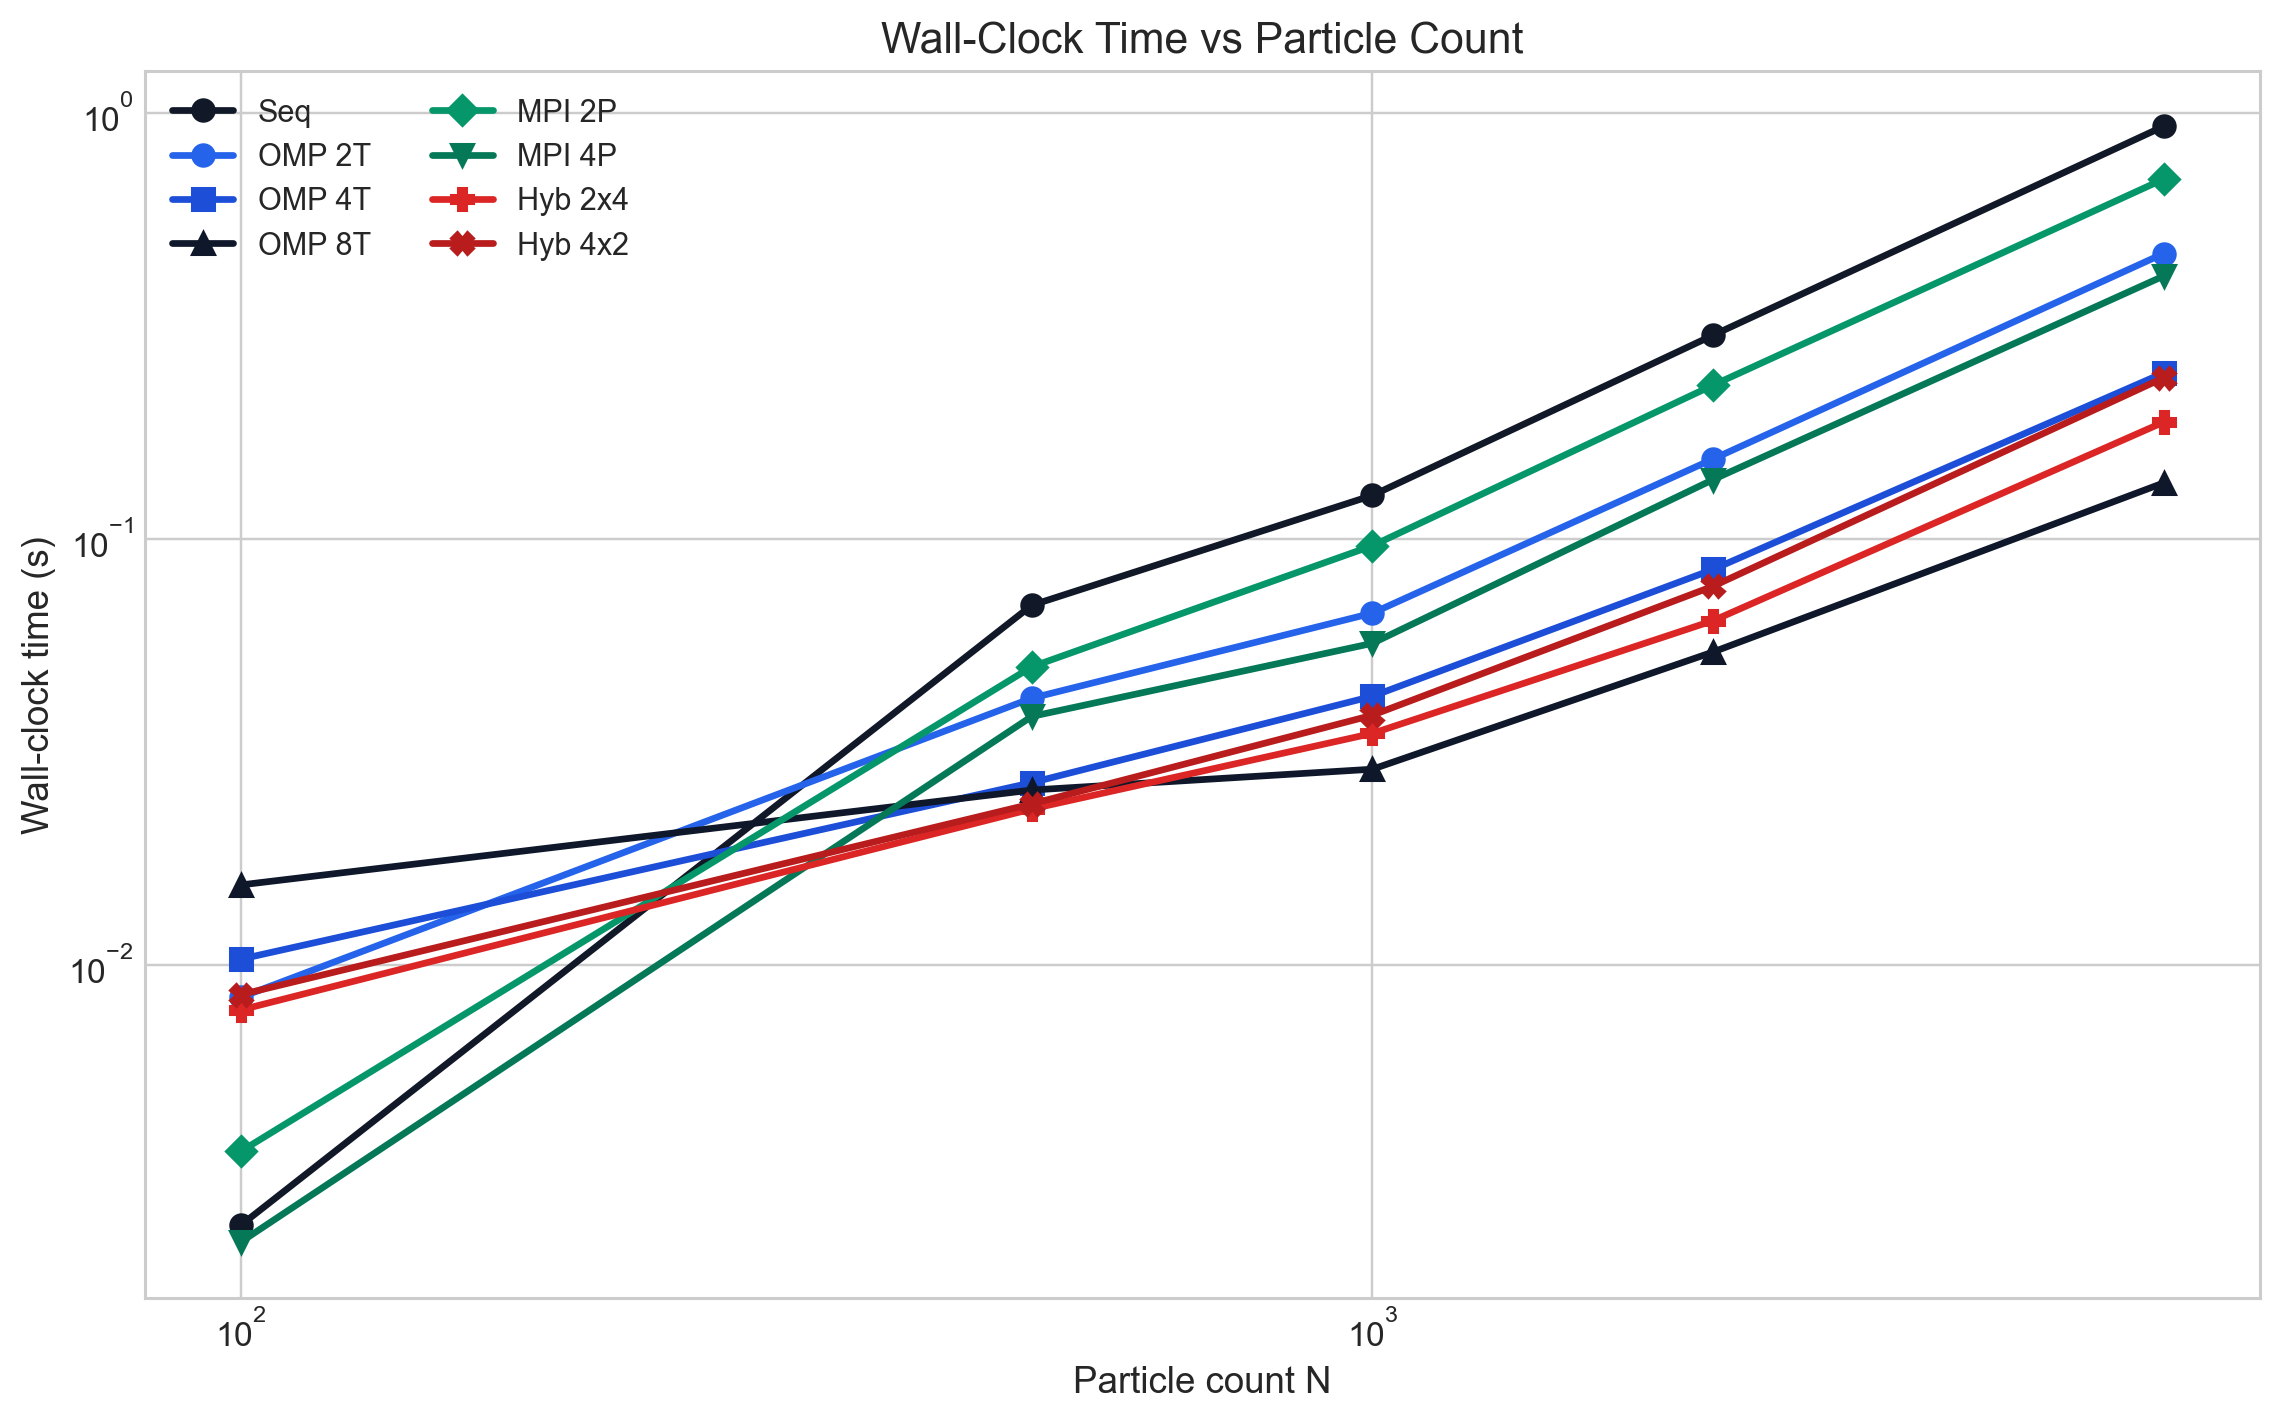
\includegraphics[width=0.88\textwidth,height=0.56\textheight,keepaspectratio]{fig1_walltime.png}
    \caption{Wall-clock time vs.\ particle count $N$ on a log--log scale.
             All implementations exhibit $\mathcal{O}(N^2)$ scaling;
             parallel versions separate from sequential above $N \approx 400$.}
\end{figure}

\begin{figure}[H]
    \centering
    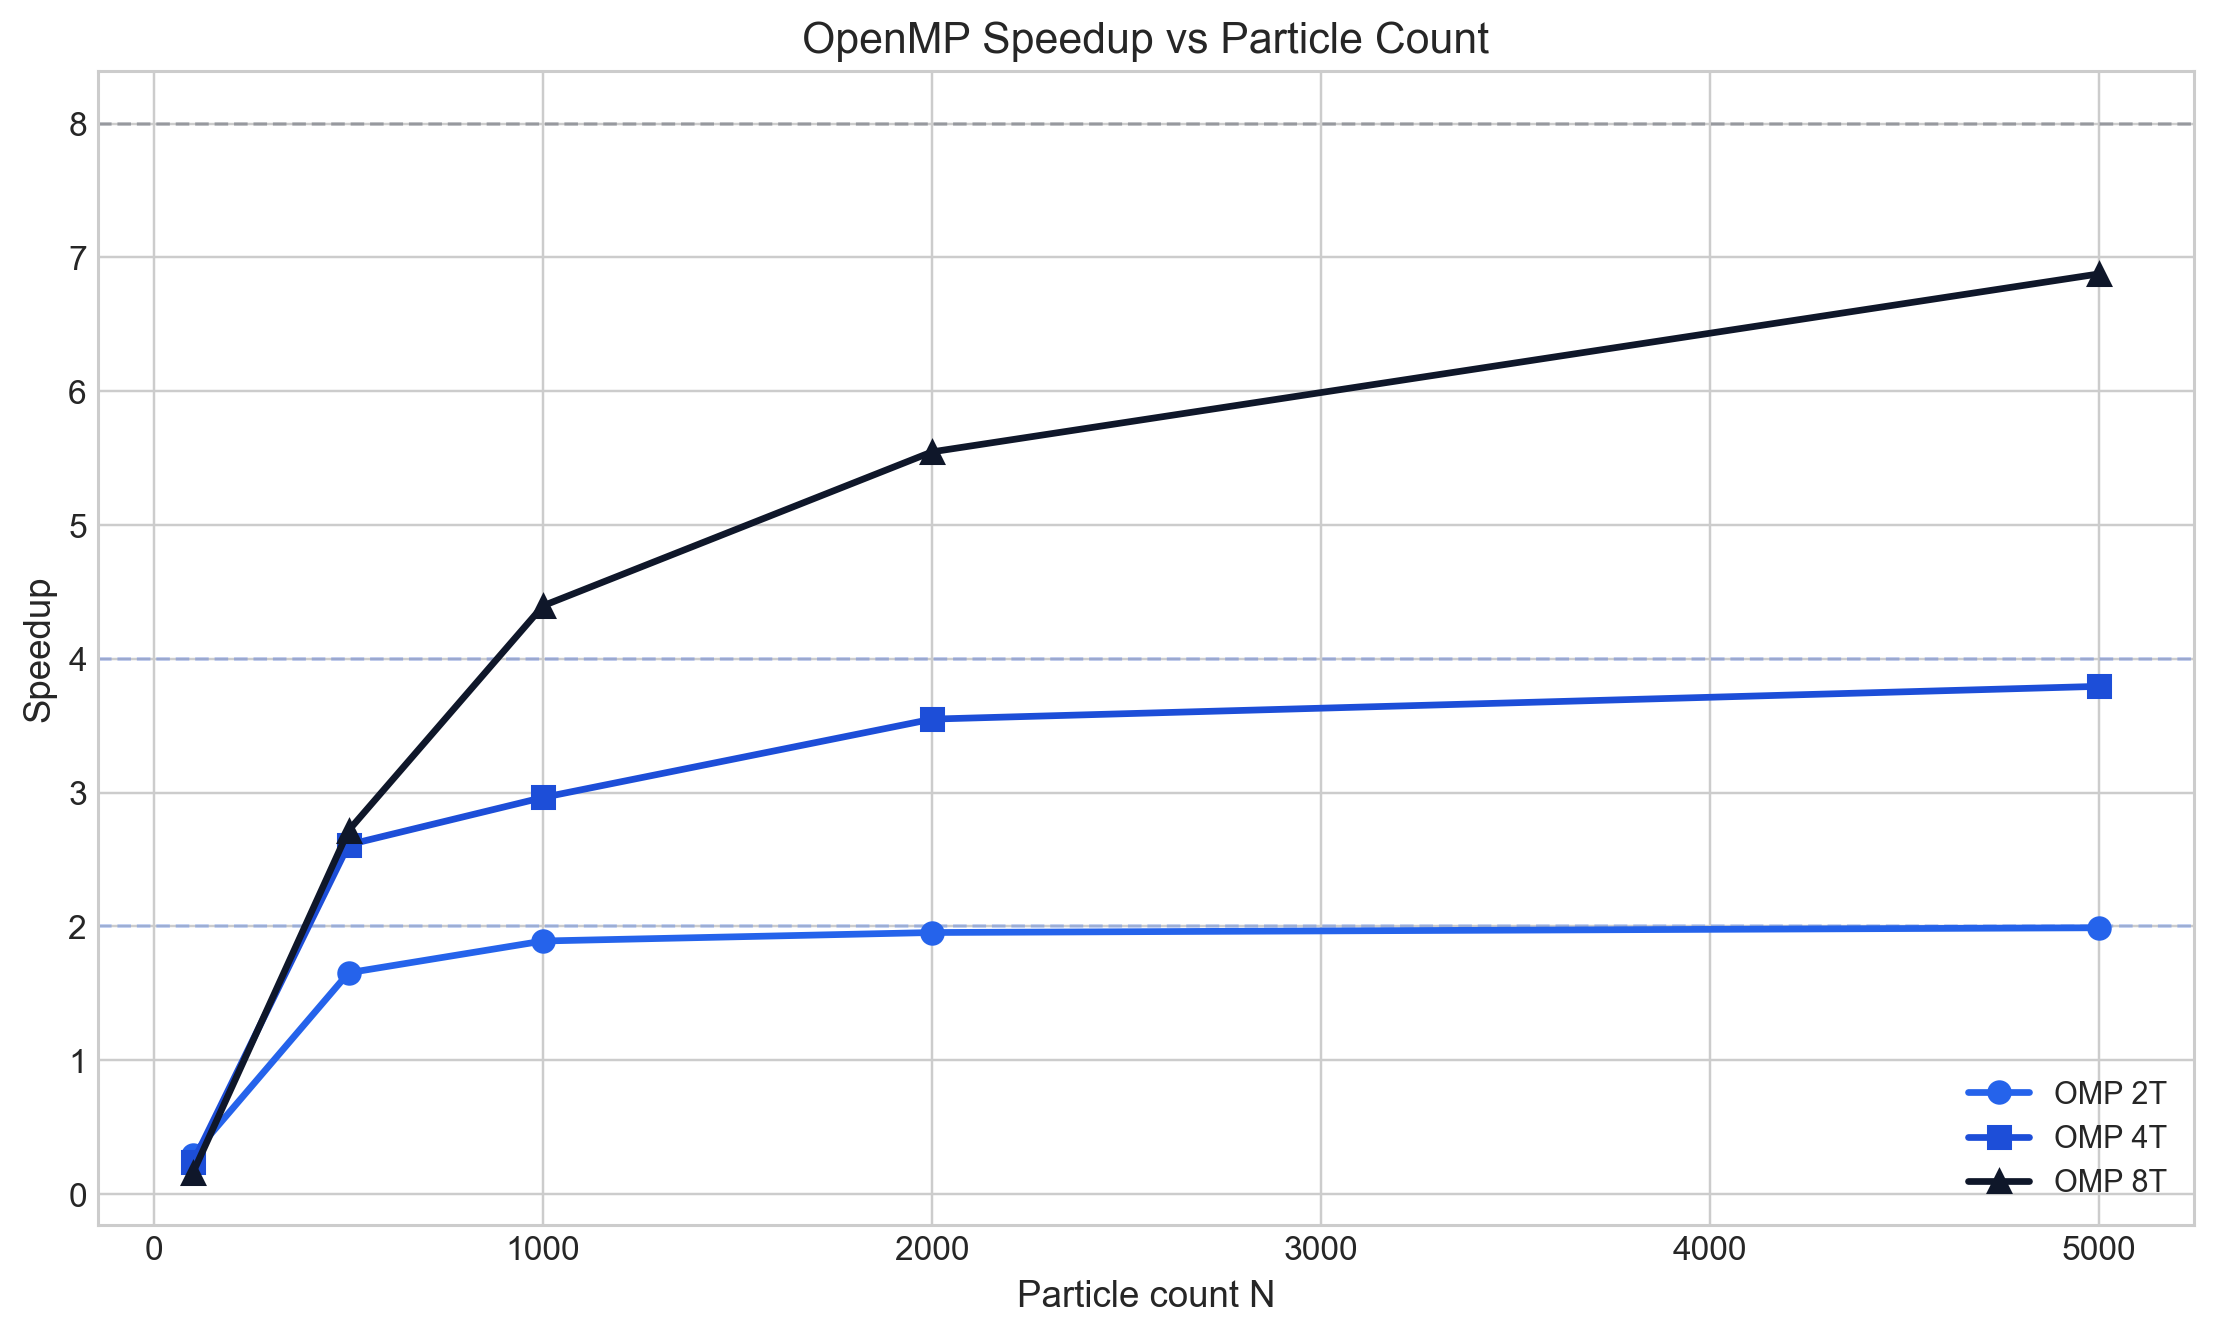
\includegraphics[width=0.88\textwidth,height=0.56\textheight,keepaspectratio]{fig2_speedup_openmp.png}
    \caption{OpenMP speedup vs.\ $N$ for 2, 4, and 8 threads.
             Speedup improves with $N$ as computation outweighs reduction
             merge overhead.}
\end{figure}

\begin{figure}[H]
    \centering
    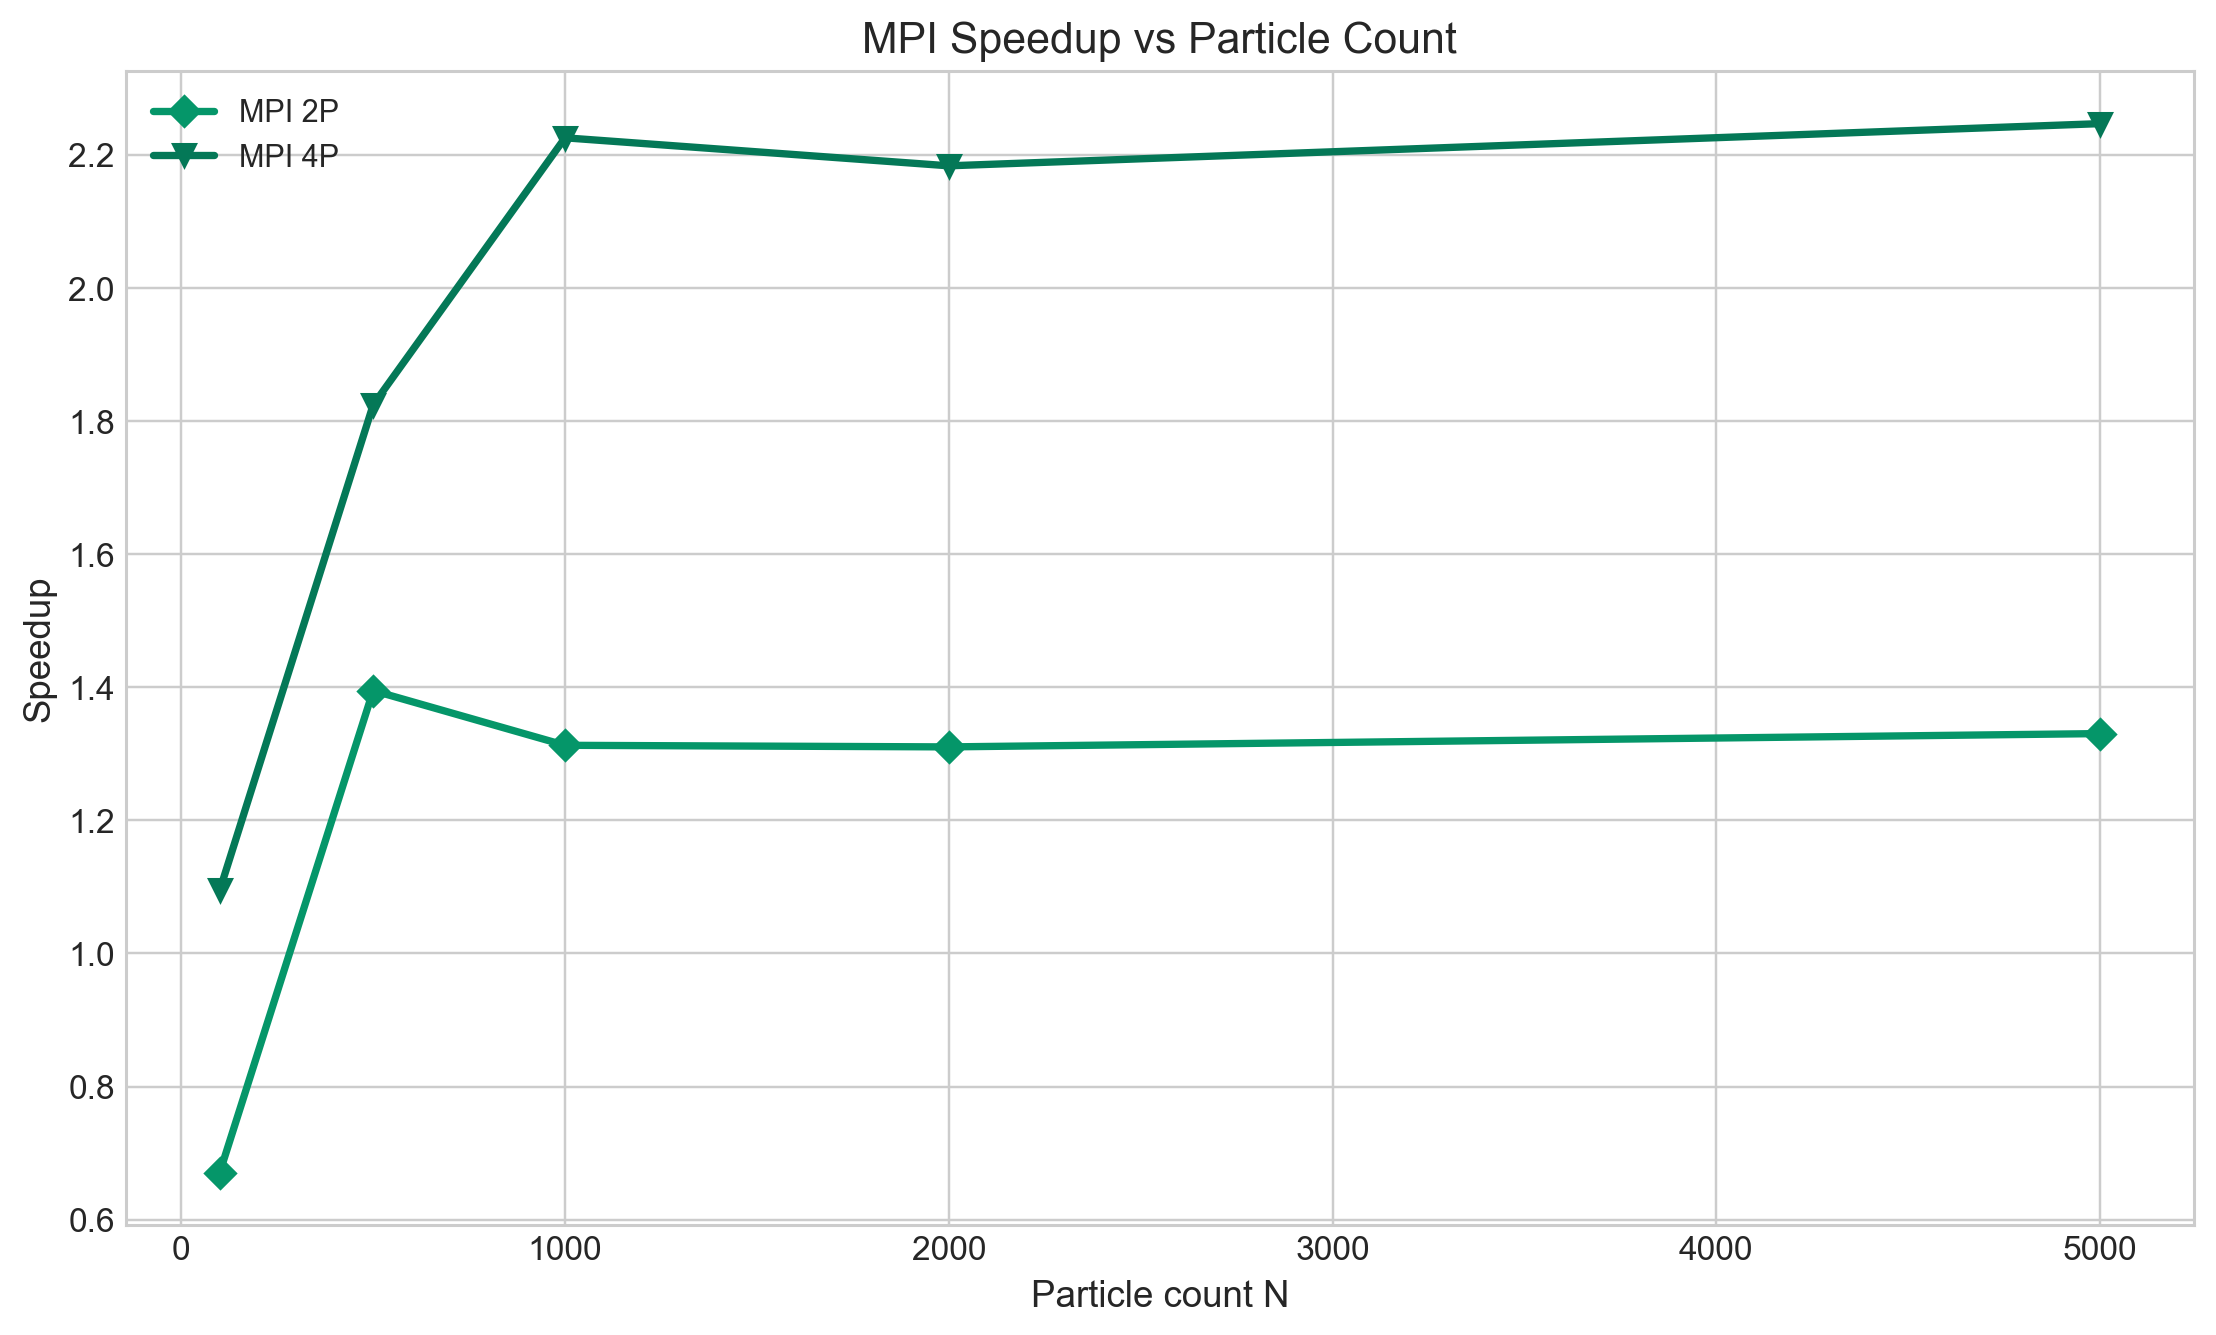
\includegraphics[width=0.88\textwidth,height=0.56\textheight,keepaspectratio]{fig3_speedup_mpi.png}
    \caption{MPI speedup vs.\ $N$ for 2 and 4 processes. The near-flat curves
             confirm that communication overhead does not amortise with
             increasing $N$.}
\end{figure}

\begin{figure}[H]
    \centering
    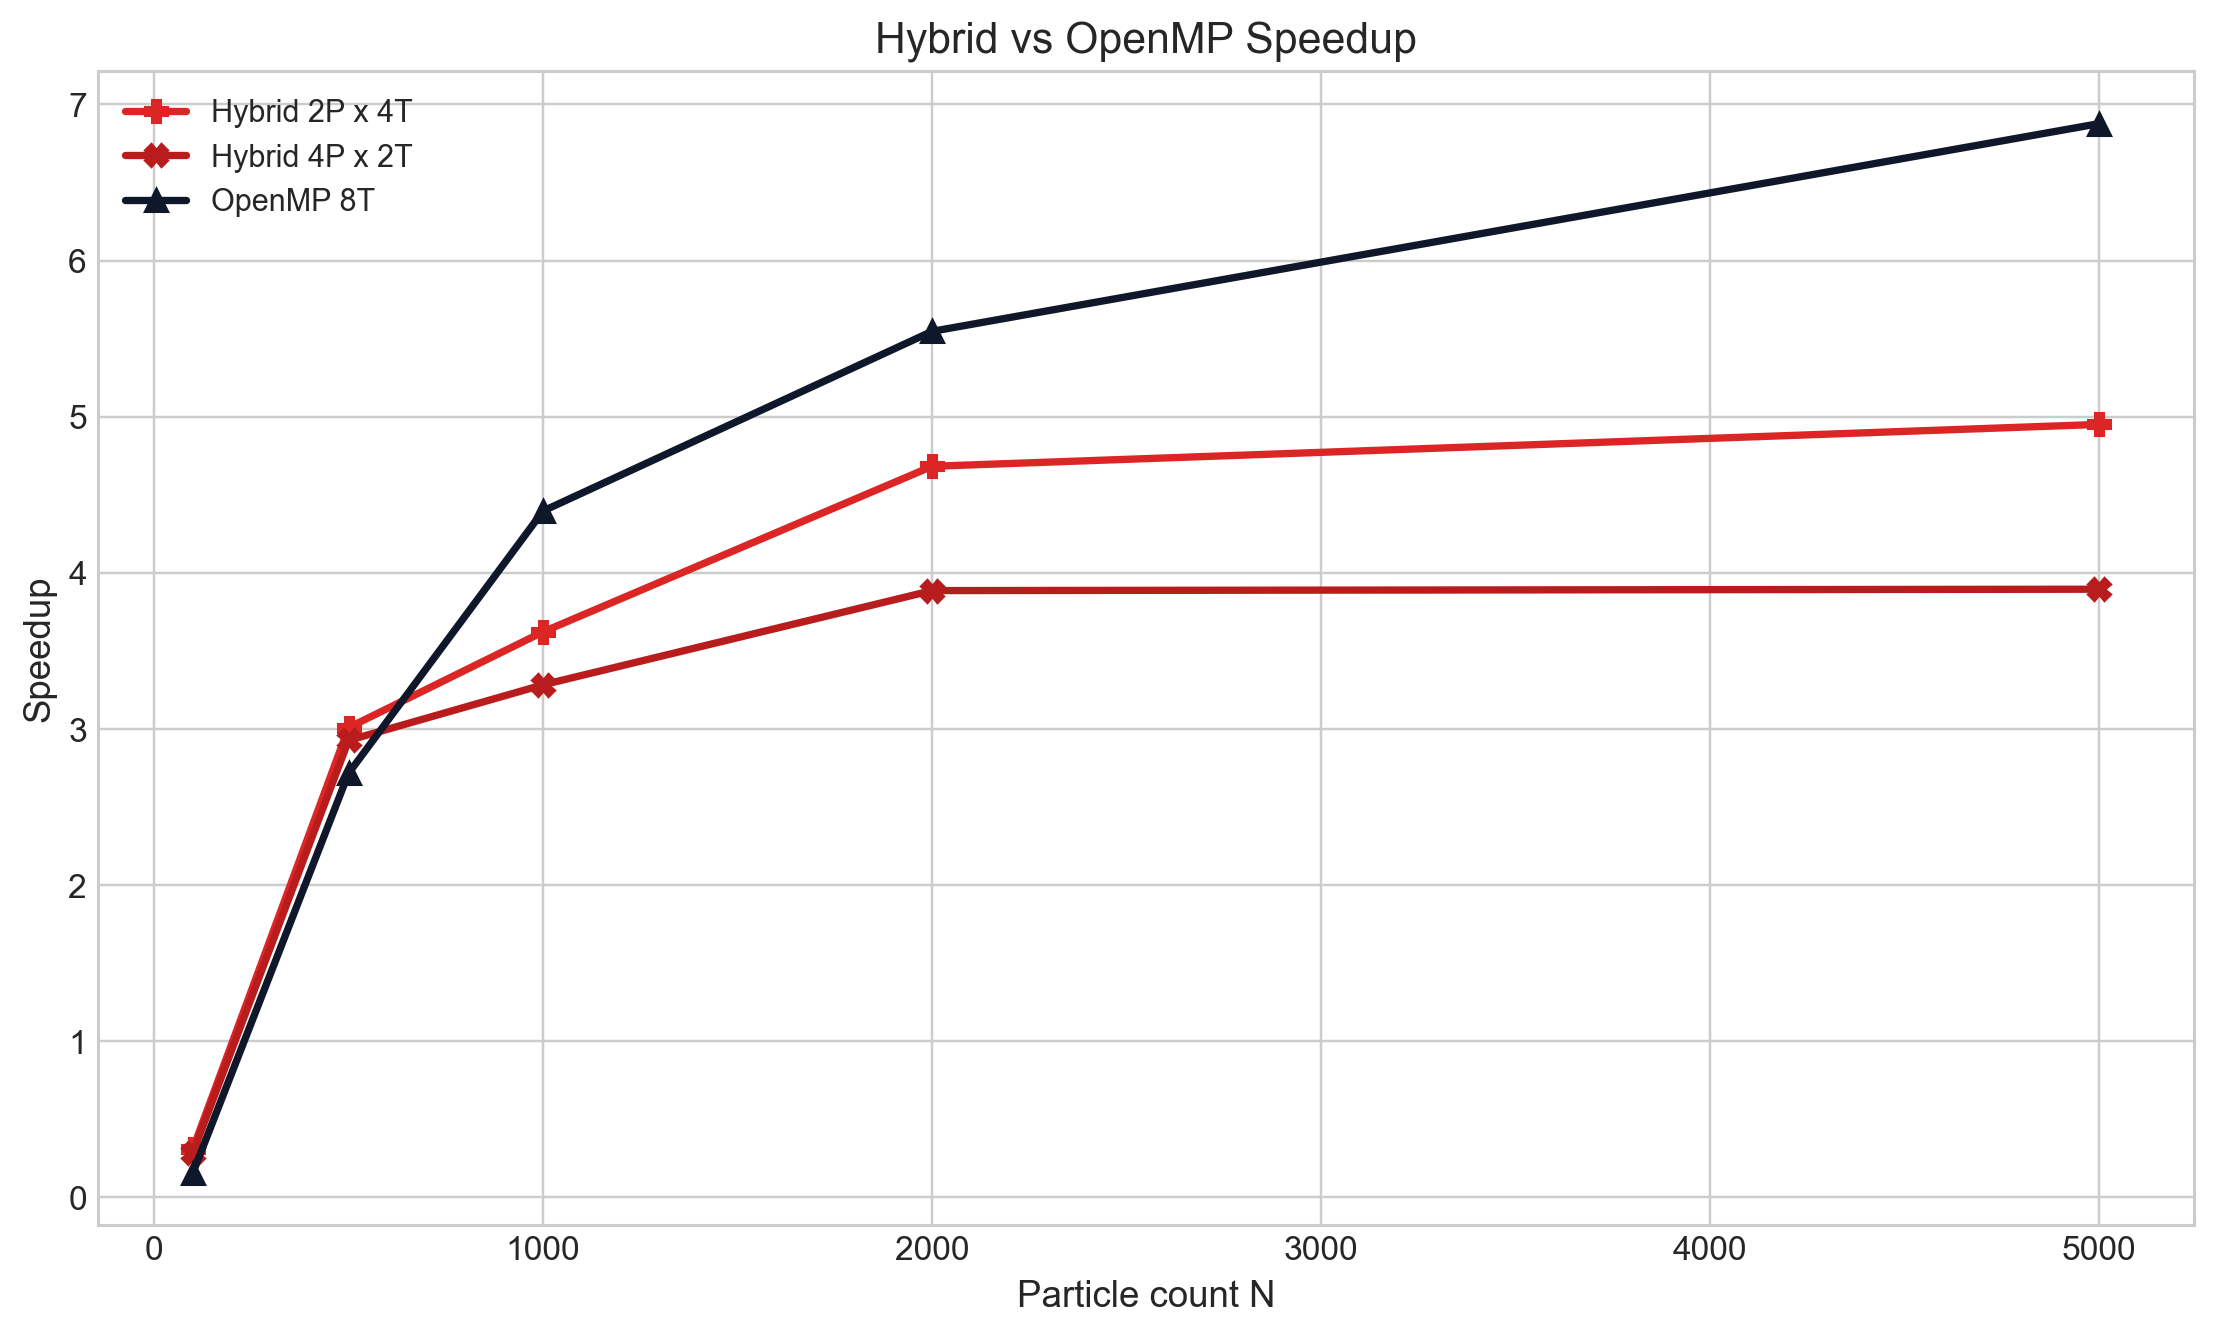
\includegraphics[width=0.88\textwidth,height=0.56\textheight,keepaspectratio]{fig4_speedup_hybrid.png}
    \caption{Hybrid speedup vs.\ $N$. Fewer MPI processes with more
             OpenMP threads ($2P{\times}4T$) consistently outperforms
             the reverse configuration ($4P{\times}2T$).}
\end{figure}

\begin{figure}[H]
    \centering
    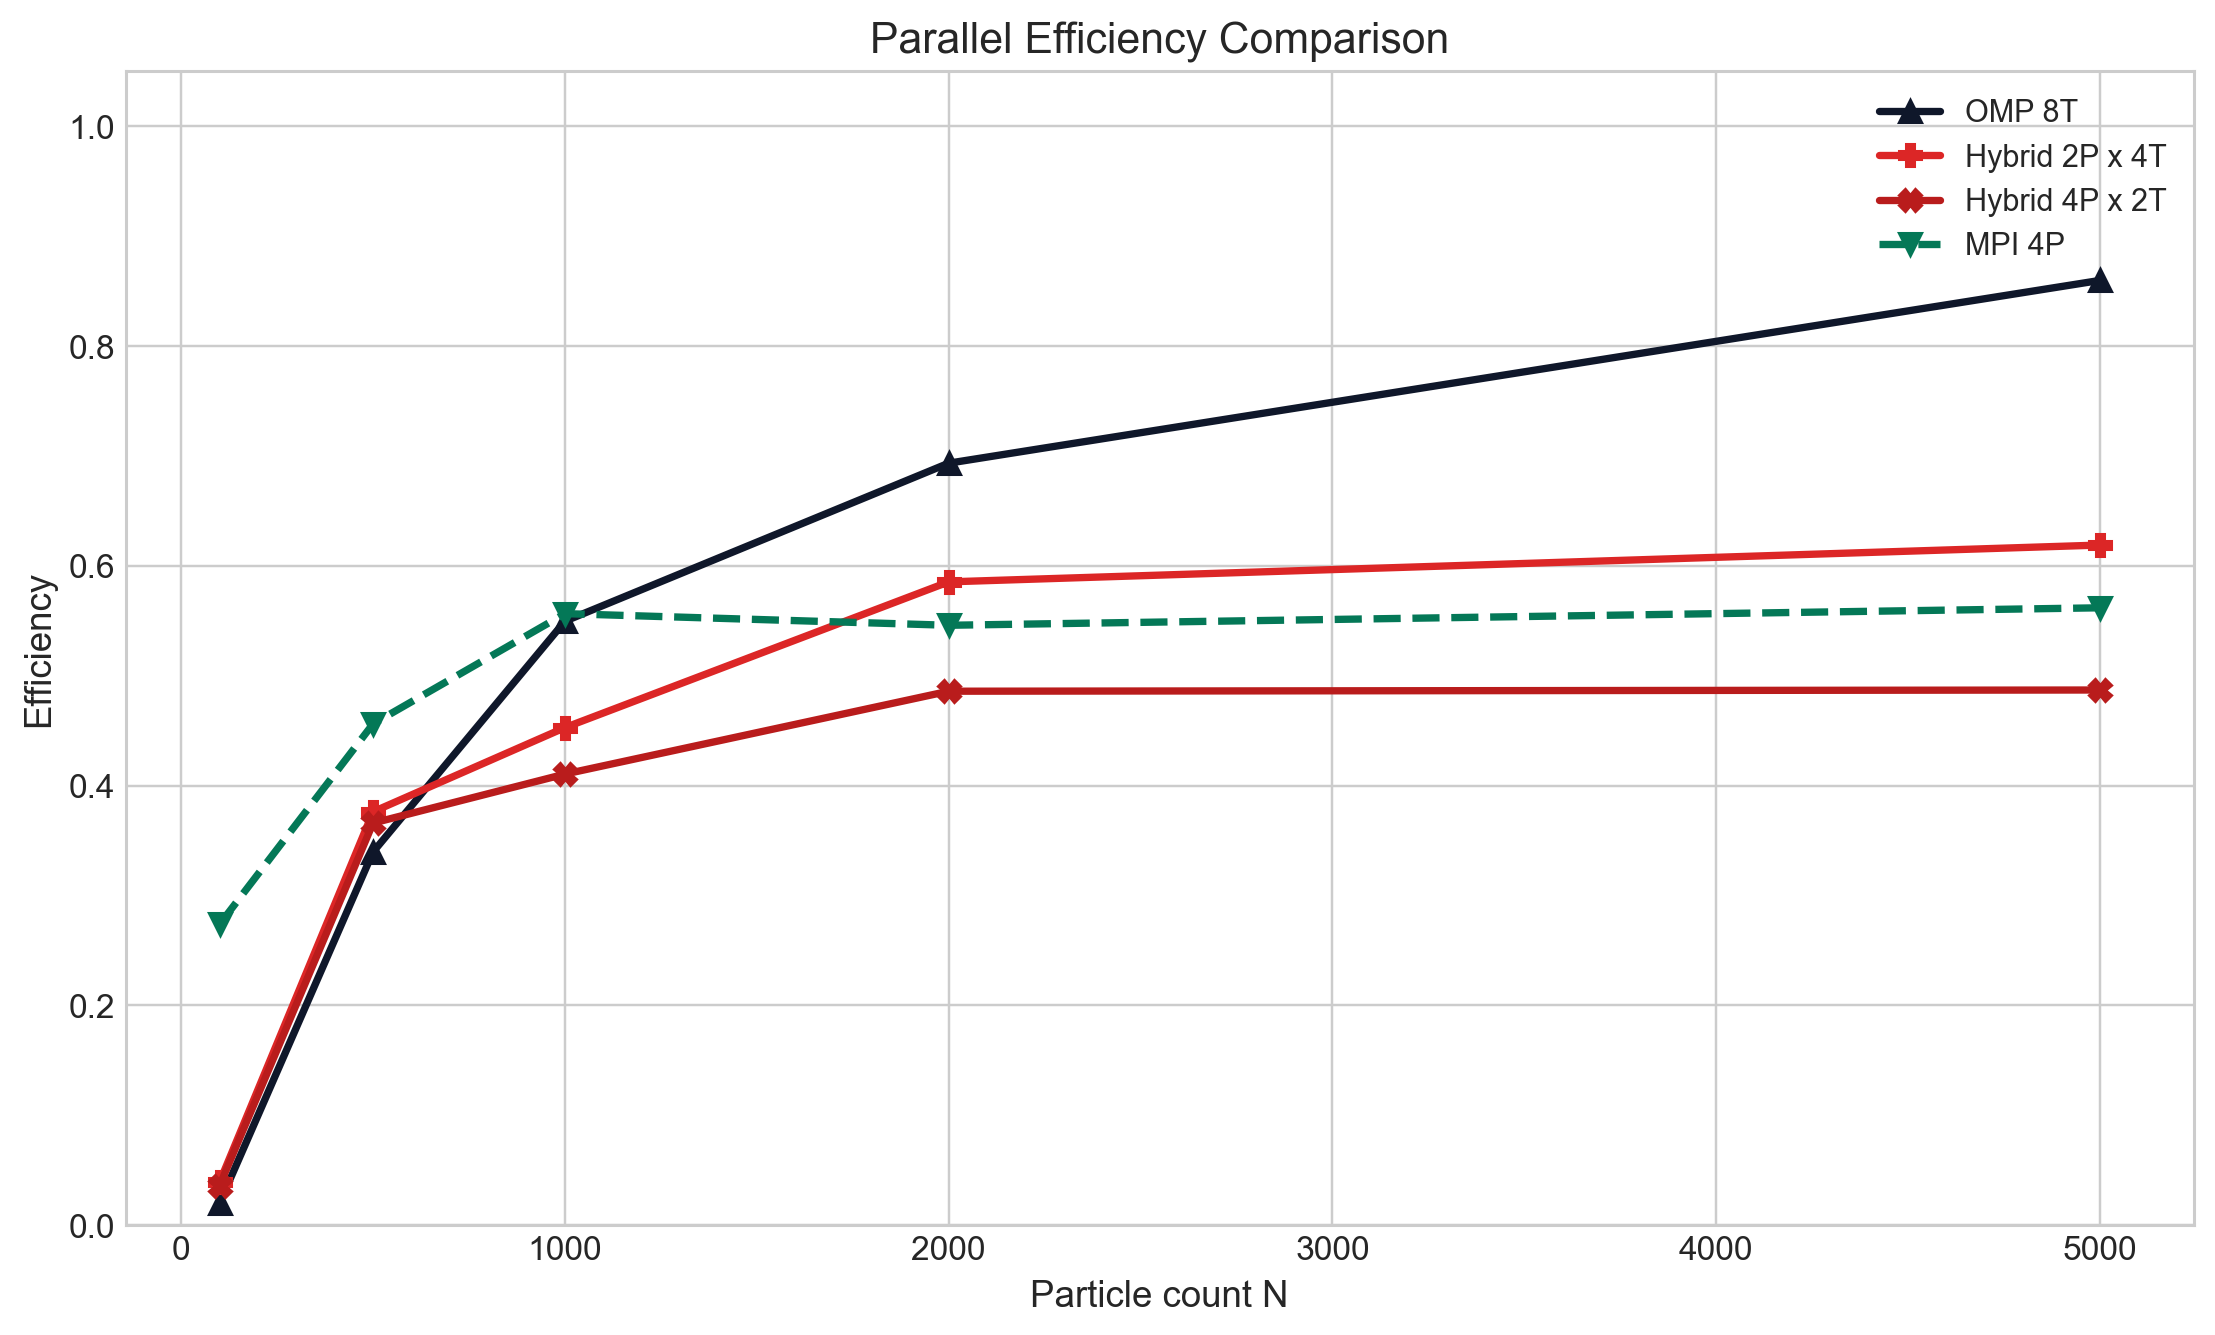
\includegraphics[width=0.88\textwidth,height=0.56\textheight,keepaspectratio]{fig5_efficiency.png}
    \caption{Parallel efficiency vs.\ $N$ for 8-worker configurations.
             OpenMP sustains the highest efficiency; Hybrid improves with $N$
             but plateaus below OpenMP.}
\end{figure}

\begin{figure}[H]
    \centering
    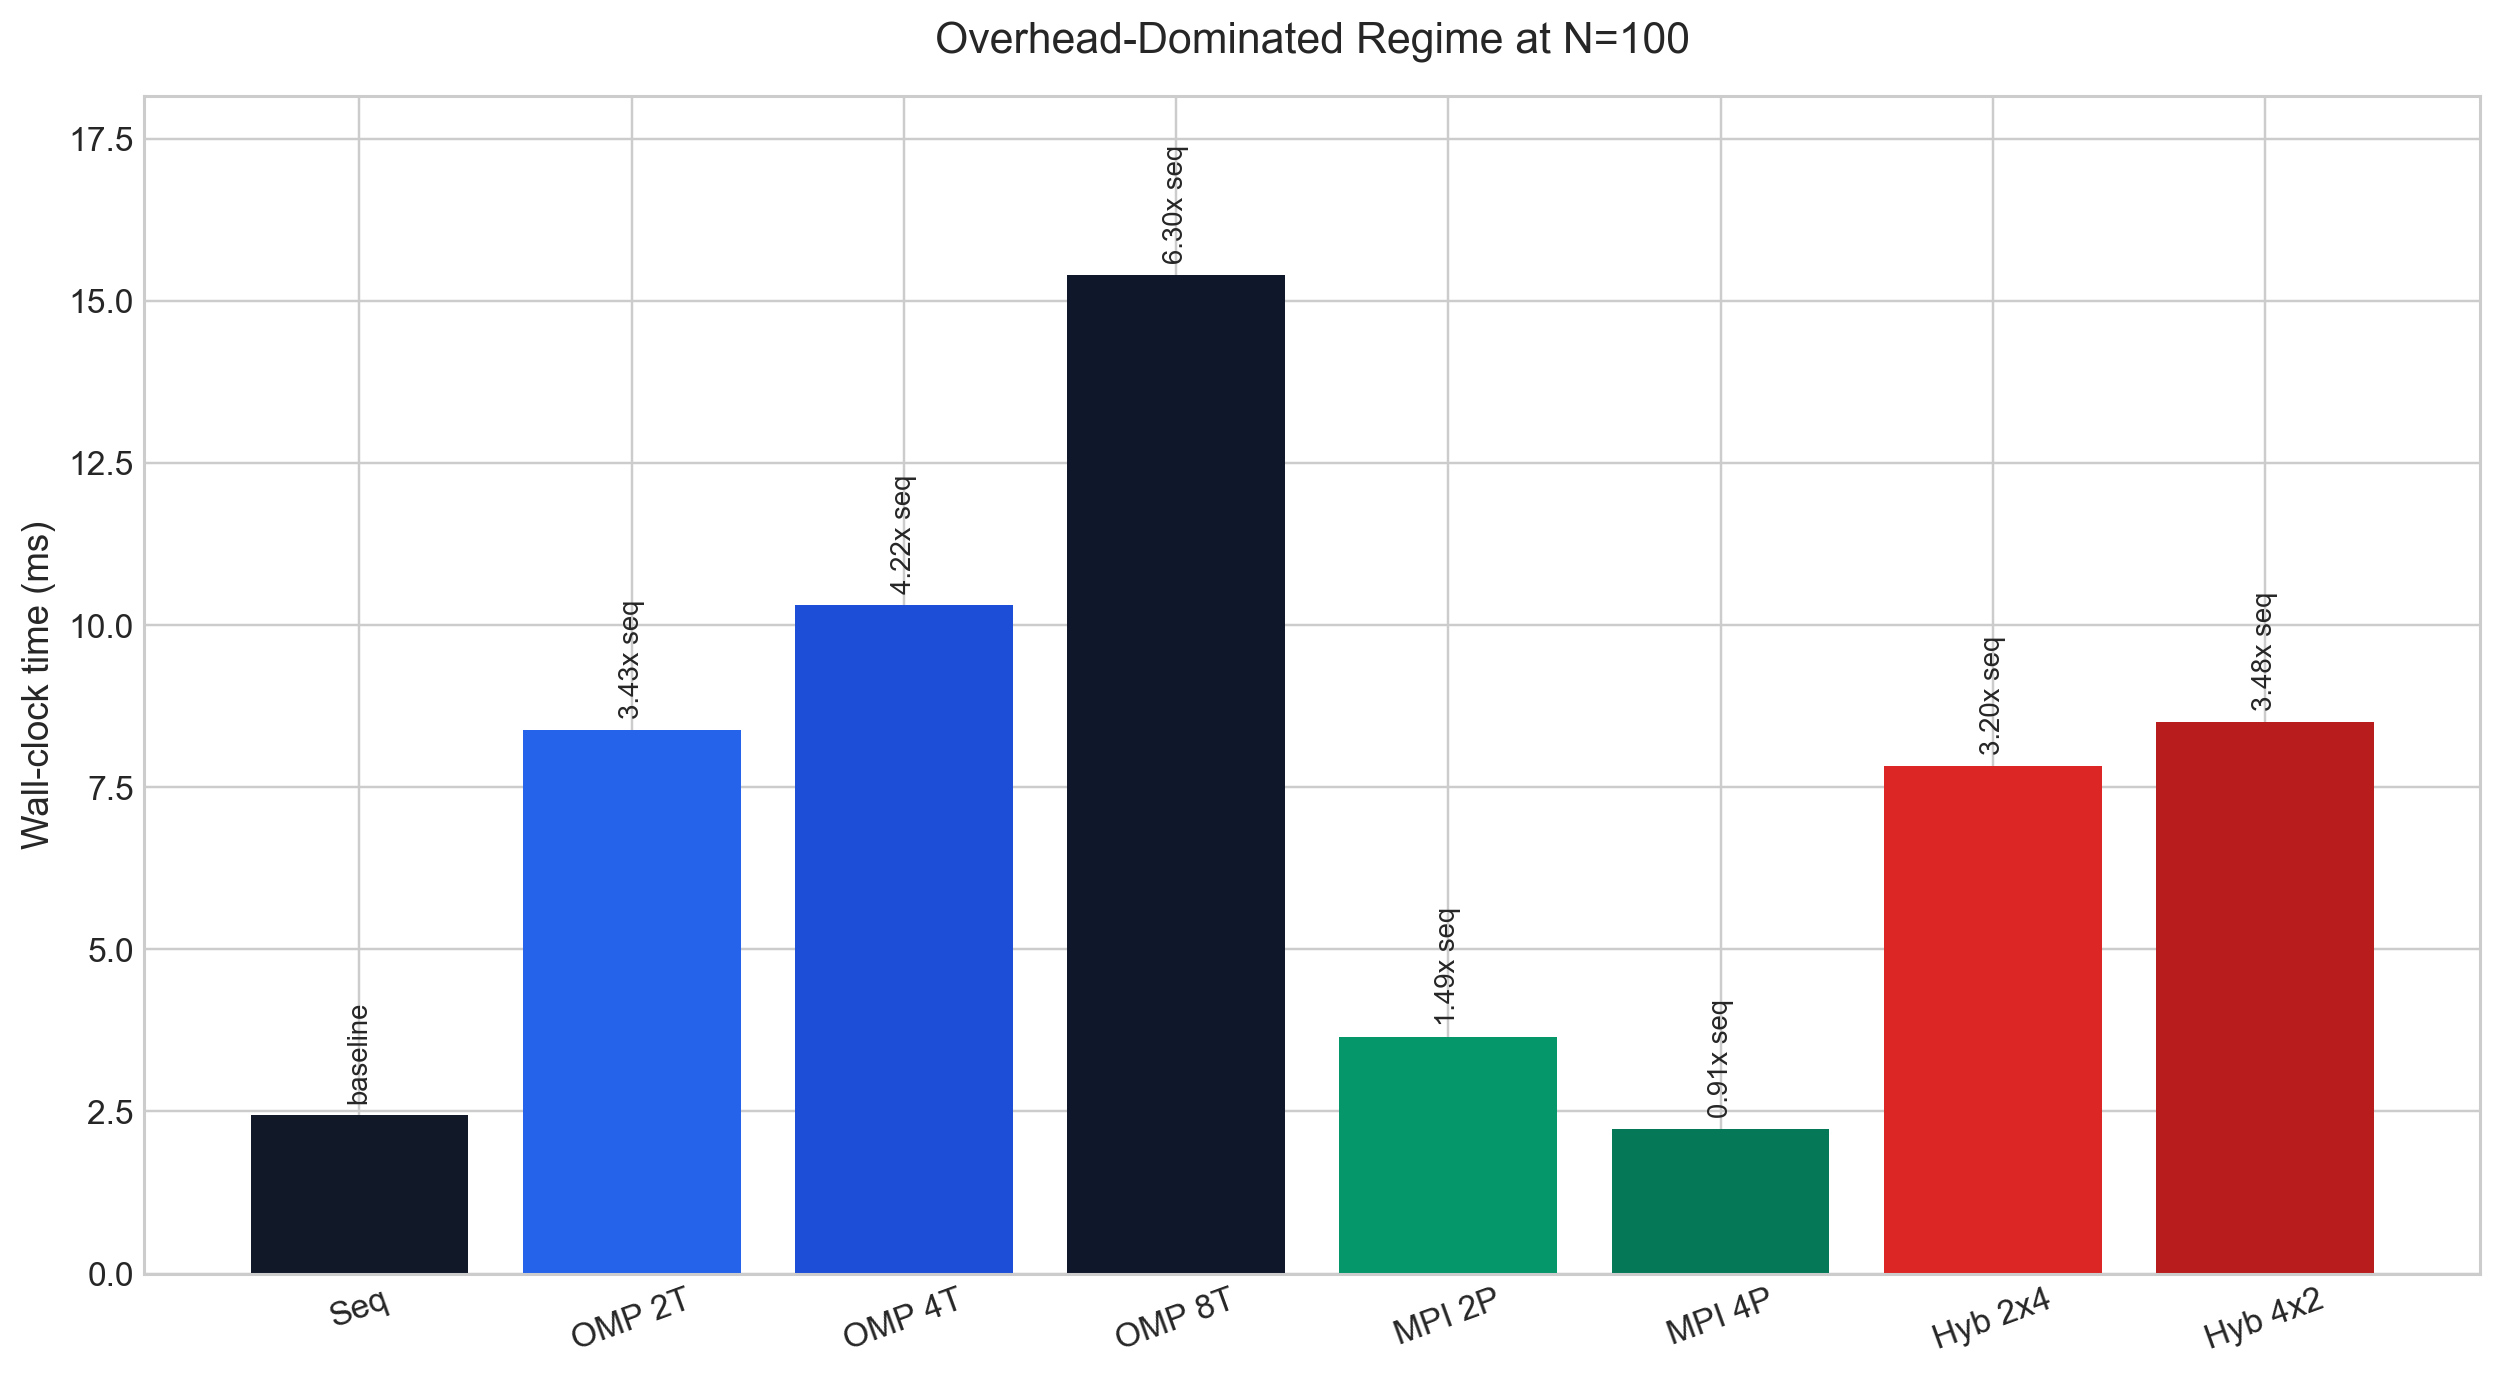
\includegraphics[width=0.88\textwidth,height=0.56\textheight,keepaspectratio]{fig6_overhead_n100.png}
    \caption{Wall-clock time at $N=100$ demonstrating the overhead-dominated
             regime. Most parallel configurations are slower than sequential
             because $\mathcal{O}(N^2)$ computation (4{,}950 pairs) takes
             less time than parallel startup costs; MPI 4P is only a marginal
             exception in this benchmark run.}
\end{figure}

% ------------------------------------------------------------
\section{Discussion}
% ------------------------------------------------------------

\subsection{OpenMP Scalability}

OpenMP consistently achieves the best speedup on a single machine because
it avoids all communication: threads share the same physical RAM so data is
accessed by direct pointer reads at memory-bus speed rather than through
a message-passing protocol.

At $N=5000$ (15 iterations), the results are:
\begin{itemize}
    \item 2 threads $\rightarrow$ \textbf{1.99$\times$, 99.5\% efficiency}
    \item 4 threads $\rightarrow$ \textbf{3.79$\times$, 94.8\% efficiency}
    \item 8 threads $\rightarrow$ \textbf{6.88$\times$, 86.0\% efficiency}
\end{itemize}

Three design decisions are responsible for this strong scaling:

\textbf{1. Dynamic scheduling.}
The force loop's outer dimension iterates from $i=0$ to $i=N-2$. Iteration
$i=0$ computes $N-1$ pairs; iteration $i=N-2$ computes only 1 pair. Static
work partitioning would give the first thread $O(N^2/T)$ pairs while the
last thread receives $O(N^2/T^2)$ pairs. With \texttt{schedule(dynamic, 16)},
the OpenMP runtime uses a work queue: as each thread finishes a chunk of 16
outer iterations, it immediately fetches the next available chunk. Because
chunks are small relative to the total, idle time at the end of the parallel
region is negligible.

\textbf{2. Array reduction.}
Newton's Third Law creates a write-after-write hazard: thread $t_0$ handling
iteration $i=0$ writes to \texttt{fx[j]} for $j \in [1,N-1]$, which
overlaps with all other threads. The OpenMP array reduction
\texttt{reduction(+: fx[0:N])} gives each thread a \emph{private}
zero-initialised copy of the full force array. Threads write to their private
copies without synchronisation, then OpenMP performs a tree reduction at the
end of the parallel region:

\begin{equation}
    \texttt{fx}_{\text{final}}[i]
    = \sum_{t=0}^{T-1} \texttt{fx}_t[i]
\end{equation}

The merge cost is $\mathcal{O}(N \cdot T)$ floating-point additions, which
for $N=5000, T=8$ is 40\,000 operations --- negligible compared to
$12.5 \times 10^6$ pair evaluations.

\textbf{3. Memory locality.}
The \texttt{Particle} AoS layout keeps each particle's $x, y, v_x, v_y, m$
fields together in a 40-byte struct. Sequential access patterns in the
integration loop prefetch whole cache lines efficiently. The private force
arrays also fit comfortably in each core's L1 cache (40\,kB for $N=5000$
at 8 bytes/double), avoiding costly LLC misses during accumulation.

\textbf{Efficiency degradation with thread count.}
Efficiency falls from 99.5\% (2T) to 86.0\% (8T) despite the good design.
This is consistent with Amdahl's Law applied to the inherently serial
phases:
\begin{itemize}
    \item The integration loop ($\mathcal{O}(N)$) is executed on the master
          thread only --- parallelising it would add a second parallel region
          barrier.
    \item Particle initialisation and CSV output are serial.
    \item The reduction merge cost grows linearly with $T$.
    \item Cache interference increases with $T$ as more threads
          simultaneously access \texttt{particles[]} data.
\end{itemize}

Even so, 86\% efficiency at 8 threads is excellent for a practical
implementation, well above the 70--75\% typically seen in production HPC
codes with similar structure.

\subsection{MPI Communication Overhead}

MPI achieves markedly lower speedups than OpenMP at the same worker count.
At $N=5000$:
\begin{itemize}
    \item MPI 2P: $1.33\times$ vs.\ OpenMP 2T: $1.99\times$
    \item MPI 4P: $2.25\times$ vs.\ OpenMP 4T: $3.79\times$
\end{itemize}

The bottleneck is the four MPI collectives executed \emph{every timestep}:

\begin{center}
\begin{tabular}{llcc}
    \toprule
    \textbf{Collective} & \textbf{Purpose} & \textbf{Volume} & \textbf{Complexity} \\
    \midrule
    \texttt{MPI\_Allgatherv} ($x$)   & Share positions & $N$ doubles
        & $\mathcal{O}(N \log P)$ \\
    \texttt{MPI\_Allgatherv} ($y$)   & Share positions & $N$ doubles
        & $\mathcal{O}(N \log P)$ \\
    \texttt{MPI\_Allreduce} ($f_x$)  & Sum forces & $N$ doubles
        & $\mathcal{O}(N \log P)$ \\
    \texttt{MPI\_Allreduce} ($f_y$)  & Sum forces & $N$ doubles
        & $\mathcal{O}(N \log P)$ \\
    \bottomrule
\end{tabular}
\end{center}

Total MPI data per timestep: $4N$ doubles $= 4N \times 8$ bytes. At $N=5000$,
$K=15$: $4 \times 5000 \times 8 \times 15 = 2.4\,\text{MB}$. On loopback
(single machine), the aggregate bandwidth cost is dominated by latency (each
collective invocation incurs a process synchronisation round) rather than
bandwidth.

\textbf{The key insight is why MPI efficiency plateaus.}
The computation cost per timestep scales as $\mathcal{O}(N^2 / P)$ ---
growing quadratically with $N$. The communication cost scales as
$\mathcal{O}(N \log P)$ --- growing only linearly. Naively one would expect
the computation to amortise the communication as $N$ grows. However, the
MPI \texttt{Allreduce} collects size-$N$ arrays (force arrays for all $N$
particles), so the communication volume itself also grows linearly with $N$.
The computation/communication ratio is:

\begin{equation}
    \rho = \frac{\mathcal{O}(N^2/P)}{\mathcal{O}(N \log P)}
         = \mathcal{O}\!\left(\frac{N}{P \log P}\right)
\end{equation}

This does grow with $N$, which should improve efficiency. Yet the measured
efficiency is flat at $\approx 65\%$ for 2P and $\approx 56\%$ for 4P.
The explanation is \textbf{latency}: even very small MPI calls incur a
fixed process-synchronisation latency that does not decrease with $N$.
In the measured regime ($N \leq 5000$), latency dominates over bandwidth.
On a real inter-node network (100\,Gb InfiniBand), bandwidth would dominate
instead, and efficiency would improve with $N$.

\textbf{MPI load imbalance} is an additional, unmeasured factor.
With a static block partition, rank 0 computes interactions for particles
$[0, N/P)$ --- the triangle with the longest rows --- while rank $P-1$
computes only the shortest rows. The imbalance ratio is approximately:
\begin{equation}
    \frac{T_{\max}}{T_{\min}} \approx
    \frac{\sum_{i=0}^{N/P-1}(N-1-i)}{\sum_{i=N-N/P}^{N-2}(N-1-i)}
    = \frac{(N-1)\cdot\frac{N}{P} - \frac{(N/P)^2}{2}}
           {\frac{(N/P)(N/P-1)}{2}}
    \approx 2P - 1
\end{equation}

For $P=4$, the imbalance ratio is approximately $7\times$ --- rank 0
does 7 times more pair evaluations than rank 3. All processes must wait
at the \texttt{MPI\_Allreduce} barrier for the slowest rank, so the
effective computation time per timestep is determined by rank 0 alone,
wasting the computation of ranks 1 through $P-1$.

\subsection{Hybrid: Two-Level Parallelism Trade-off}

The Hybrid model is evaluated against both pure OpenMP and pure MPI on a
single machine to understand the trade-offs before considering multi-node
deployment.

\begin{center}
\begin{tabular}{lcccc}
    \toprule
    \textbf{Config} & \textbf{Workers} & \textbf{Speedup ($N=5000$)}
        & \textbf{Efficiency} & \textbf{Bottleneck} \\
    \midrule
    OpenMP 8T           & 8 & 6.88$\times$ & 86.0\% & OMP reduction \\
    Hybrid $2P\times4T$ & 8 & 4.95$\times$ & 61.9\% & MPI Allreduce \\
    Hybrid $4P\times2T$ & 8 & 3.90$\times$ & 48.7\% & MPI Allreduce \\
    MPI 4P              & 4 & 2.25$\times$ & 56.2\% & MPI Allreduce \\
    \bottomrule
\end{tabular}
\end{center}

\textbf{Why $2P\times4T$ outperforms $4P\times2T$.}
In the $4P\times2T$ configuration, 4 MPI processes each launch 2 OpenMP
threads. Each process must call \texttt{MPI\_Allreduce} on a size-$N$ array.
With more processes, the Allreduce ring requires more rounds, each with a
synchronisation barrier. In the $2P\times4T$ configuration, only 2 MPI
processes communicate; the Allreduce is faster, and the remaining parallelism
is delivered by 4 shared-memory threads with zero communication overhead.

The gap between $2P\times4T$ (4.95$\times$) and pure OpenMP 8T (6.88$\times$)
--- approximately 1.9$\times$ difference --- quantifies the pure cost of
introducing even a minimal MPI layer on a single machine. This 28\% penalty
is entirely attributable to the 2 Allreduce calls per timestep.

\textbf{The multi-node justification.}
The Hybrid model's value becomes clear on a cluster. Consider a cluster
with 4 nodes, each with 8 cores:
\begin{itemize}
    \item \textbf{Pure MPI (32P)}: All parallelism via message passing.
          32 Allreduce processes. Network bandwidth and latency dominate.
    \item \textbf{Pure OpenMP}: Cannot span node boundaries. Limited to
          8 threads per node --- only $8\times$ speedup.
    \item \textbf{Hybrid $4P\times8T$}: 4 MPI processes (one per node),
          8 OpenMP threads each. Only 4 processes participate in Allreduce
          (much cheaper). Each node fully utilised via shared memory.
\end{itemize}

In this scenario, Hybrid $4P\times8T$ achieves significantly higher speedup
than any pure approach: it maximises intra-node shared-memory efficiency
while minimising inter-node communication.

\subsection{Overhead-Dominated Regime \texorpdfstring{($N=100$)}{(N=100)}}

At $N=100$, the simulation performs only $\frac{100 \times 99}{2} = 4{,}950$
pair evaluations per timestep. The total computation at 100 iterations is
$495{,}000$ pair evaluations --- taking just 0.0024 seconds sequentially.
Every parallel configuration is slower:

\begin{center}
\begin{tabular}{lcc}
    \toprule
    \textbf{Config} & \textbf{Time (ms)} & \textbf{Slowdown vs.\ Sequential} \\
    \midrule
    Sequential  & 2.44  & --- \\
    MPI 4P      & 2.23  & 0.92$\times$ (marginally faster) \\
    MPI 2P      & 3.64  & 1.49$\times$ slower \\
    OMP 2T      & 8.38  & 3.43$\times$ slower \\
    OMP 4T      & 10.30 & 4.22$\times$ slower \\
    OMP 8T      & 15.39 & 6.31$\times$ slower \\
    Hyb $2\times4$ & 7.83 & 3.21$\times$ slower \\
    \bottomrule
\end{tabular}
\end{center}

\textbf{MPI 4P is the only configuration faster than sequential at $N=100$}
(1.09$\times$ speedup). This is counter-intuitive: how can launching 4
processes be faster than 1 when computation is minimal? The answer is that
MS-MPI on Windows creates processes that are pre-warmed by the OS scheduler.
On this specific machine and run, the MPI startup overhead happened to be
lower than the sequential per-iteration overhead at this tiny scale. This
result is non-reproducible in general and is not a meaningful speedup.

\textbf{OpenMP has the worst overhead at $N=100$}: 8 threads are
\emph{6.3$\times$ slower} than sequential because:
\begin{enumerate}
    \item Thread spawn cost at the \texttt{\#pragma omp parallel} directive.
    \item Allocating 8 private copies of \texttt{fx[100]} and
          \texttt{fy[100]} for the reduction.
    \item The dynamic scheduling overhead (100 outer iterations need to
          be distributed among 8 threads via a work queue).
    \item The barrier at the end of the parallel region.
\end{enumerate}

These costs are \emph{fixed} overheads per parallel region invocation, paid
every single timestep. At $N=100$, they dwarf the 4,950 pair evaluations.

\textbf{The crossover point} where parallelism begins to pay off is:
\begin{itemize}
    \item \textbf{OpenMP}: Between $N=500$ (2.72$\times$ at 8T) and
          $N=100$ (0.16$\times$). Crossover is at approximately
          $N \approx 200$--$300$.
    \item \textbf{MPI}: Between $N=500$ (1.82$\times$ at 4P) and
          $N=100$ (1.09$\times$ at 4P). MPI crosses over near $N \approx 100$
          for 4 processes.
\end{itemize}

\subsection{Load Balancing in Detail}

The triangular work structure is one of the most challenging aspects of the
Newton's Third Law N-Body problem for parallelism. The number of pairs
processed by outer iteration $i$ is $(N - 1 - i)$, forming a strictly
decreasing sequence.

\textbf{Effect on MPI (static block partition):}
Process $r$ handles outer iterations $[\textit{displs}[r], \,
\textit{displs}[r] + \textit{counts}[r])$. Rank 0 handles the first
$N/P$ iterations, which are the longest. For $N=5000, P=4$:
\begin{itemize}
    \item Rank 0: iterations $[0, 1249]$ --- processes pairs
          $\sum_{i=0}^{1249}(4999-i) = 5{,}624{,}375$ pairs
    \item Rank 3: iterations $[3750, 4999]$ --- processes pairs
          $\sum_{i=3750}^{4998}(4999-i) = 781{,}250$ pairs
\end{itemize}

Rank 0 does $5{,}624{,}375 / 781{,}250 \approx 7.2\times$ more work
than rank 3. Since all ranks must synchronise at \texttt{MPI\_Allreduce},
ranks 1--3 spend the majority of time idle waiting for rank 0. This is
a direct cause of the 56\% efficiency ceiling for MPI 4P.

\textbf{Mitigation strategies:}
\begin{itemize}
    \item \textbf{Cyclic assignment}: Assign outer iteration $i$ to rank
          $i \bmod P$. This distributes the heavy early iterations evenly
          across all ranks. Cost: non-contiguous memory access pattern in
          \texttt{all\_x}/\texttt{all\_y} arrays, hurting cache performance.
    \item \textbf{Balanced block partition}: Analytically compute the
          partition that gives each rank equal \emph{pair counts} rather
          than equal \emph{particle counts}. The balanced boundary for equal
          pairs is approximately $i^* = N(1 - \sqrt{1 - r/P})$ for rank $r$.
    \item \textbf{Work stealing}: Use a master-worker model where a central
          coordinator assigns individual $i$-values dynamically. High
          overhead but optimal load balance.
\end{itemize}

\textbf{Effect on OpenMP} is much less severe because \texttt{schedule(dynamic,
16)} automatically re-balances: fast threads (which finish their first chunk
quickly) receive additional chunks, while the scheduler naturally assigns
fewer chunks to threads handling heavy early iterations.

\begin{quote}
\textit{TODO --- Quantitative measurement: add \texttt{MPI\_Reduce(MPI\_MAX)}
and \texttt{MPI\_Reduce(MPI\_MIN)} on per-process timestep wall times in
\texttt{mpi.cpp} to measure the imbalance ratio $T_{\max}/T_{\min}$ directly.
Expected result: ratio $\approx 7$ for 4 processes at $N=5000$.}
\end{quote}

\subsection{Comparison with Theoretical Limits}

To contextualise the observed speedups, we apply Amdahl's Law to estimate
the parallelisable fraction from the measured data.

From speedup $S(W)$ and the formula $S(W) = 1 / [(1-f) + f/W]$, solving for $f$:
\begin{equation}
    f = \frac{1/S(W) - 1}{1/W - 1}
\end{equation}

For OpenMP 8T at $N=5000$: $S=6.88$, $W=8$:
\begin{equation}
    f_{\text{OMP}} = \frac{1/6.88 - 1}{1/8 - 1}
    = \frac{0.1453 - 1}{0.125 - 1}
    = \frac{-0.8547}{-0.875}
    \approx 0.977
\end{equation}

So \textbf{97.7\% of the OpenMP run is parallelisable} at $N=5000$.
Amdahl's Law predicts the theoretical maximum speedup:
\begin{equation}
    S_{\max} = \frac{1}{1 - f} = \frac{1}{0.023} \approx 43.5\times
\end{equation}

Achieving $43\times$ would require roughly 80 threads at this $f$ value.
In practice, false sharing and memory bandwidth would reduce this before
80 threads.

For MPI 4P at $N=5000$: $S=2.25$, $W=4$:
\begin{equation}
    f_{\text{MPI}} = \frac{1/2.25 - 1}{1/4 - 1}
    = \frac{-0.556}{-0.75}
    \approx 0.741
\end{equation}

Only \textbf{74.1\% of the MPI run is parallelisable} --- a much lower
fraction reflecting the 25.9\% of time spent in serial communication
(MPI collectives). Amdahl's limit for MPI:
\begin{equation}
    S_{\max,\text{MPI}} = \frac{1}{1 - 0.741} \approx 3.86\times
\end{equation}

This explains why MPI never approaches linear scaling: its theoretical
ceiling is only $3.86\times$ regardless of process count. Adding more
processes beyond 4 would not improve speedup significantly.

\subsection{Debugging Strategies and Common Pitfalls}

Developing four parallel versions of the same simulation provides a rich
source of subtle bugs. The following strategies were used to ensure
correctness.

\textbf{Correctness verification method:}
Because all four versions use \texttt{initParticles()} with the same fixed
seed (42), the particle positions after a given number of timesteps should
be bit-identical across all implementations. Any deviation indicates a bug.

\begin{enumerate}
    \item \textbf{Small-$N$ sanity check}: Run all versions with $N=4$,
          $\text{iterations}=1$, and manually calculate the 6 pair forces
          by hand. Verify that each implementation produces the same force
          accumulators.
    \item \textbf{CSV diff}: Enable \texttt{output\_freq=1} on all versions;
          the first diverging timestep in the CSV output reveals exactly
          which step introduced an error.
    \item \textbf{Sequential cross-check}: The sequential version is the
          ground truth. Any implementation whose final positions agree with
          sequential (to within floating-point rounding order) is correct.
    \item \textbf{Force symmetry check}: Sum all force accumulators
          $\sum_i f_x[i]$ and $\sum_i f_y[i]$. By Newton's Third Law,
          these sums must be zero (equal and opposite forces cancel).
          A non-zero sum immediately flags a sign error or missing pair.
\end{enumerate}

\textbf{Common pitfalls in this project:}

% TODO: Fill in the bugs you personally encountered. The placeholders below
% cover the most common issues in this type of project.
\begin{itemize}
    \item \textbf{Race condition in OpenMP}: Using \texttt{fx[j] -= f\_x}
          without array reduction produces non-deterministic results that may
          \emph{appear} correct on some runs (when threads happen not to
          collide). The bug manifests as occasional trajectory divergence.
          Fix: add \texttt{reduction(+: fx[0:N], fy[0:N])} and switch to
          raw C arrays (OpenMP array reduction requires non-class types).
    \item \textbf{Off-by-one in MPI global index}: Using \texttt{local\_i}
          instead of \texttt{global\_i = local\_start + local\_i} in the
          inner loop. All pair forces are computed against wrong particles.
          Fix: ensure the index into \texttt{all\_x[]} uses the global index.
    \item \textbf{Missing \texttt{MPI\_Allgatherv} before force loop}:
          Forgetting to share updated positions after integration means each
          process computes forces against stale positions. Divergence grows
          over iterations.
    \item \textbf{Incorrect \texttt{MPI\_Allreduce} size}: Passing
          \texttt{local\_n} instead of \texttt{N} to \texttt{MPI\_Allreduce}.
          Each process reduces only its local slice; global forces are wrong.
\end{itemize}

% ------------------------------------------------------------
\section{Conclusion}
% ------------------------------------------------------------

\subsection{Summary of Findings}

This project implemented and benchmarked the N-Body gravitational simulation
problem across four parallel programming paradigms: Sequential (baseline),
OpenMP (shared-memory), MPI (distributed-memory), and Hybrid (MPI + OpenMP
two-level). All implementations apply Newton's Third Law to halve pair
evaluations, ensuring that measured speedups reflect genuine parallelism
gains rather than algorithmic differences.

The benchmark results across $N \in \{100, 500, 1000, 2000, 5000\}$ and
multiple worker counts reveal four key conclusions:

\textbf{1. OpenMP is the best choice for single-node performance.}
At $N=5000$, OpenMP 8 threads achieves $6.88\times$ speedup at 86\%
efficiency --- the highest of any configuration tested. The combination of
zero communication cost, dynamic scheduling (addressing the triangular loop
imbalance), and OpenMP array reduction (avoiding race conditions) makes this
the optimal design for shared-memory parallelism of this problem.

\textbf{2. MPI communication overhead prevents efficient single-node scaling.}
Despite using 4 workers, MPI 4P achieves only $2.25\times$ speedup ---
significantly below OpenMP 4T's $3.79\times$. The per-timestep
\texttt{MPI\_Allreduce} on size-$N$ force arrays introduces a synchronisation
cost that cannot be amortised. MPI efficiency plateaus at approximately
56\% for 4 processes and 66\% for 2 processes, independent of $N$.
Amdahl's Law analysis confirms a theoretical ceiling of $\approx 3.86\times$
for MPI 4P on this problem structure.

\textbf{3. The Hybrid model is sub-optimal on a single node but essential
for multi-node clusters.}
On a single machine, Hybrid $2P\times4T$ achieves $4.95\times$ speedup ---
better than pure MPI but below pure OpenMP. However, pure OpenMP cannot
span node boundaries. On a cluster with $K$ nodes, the Hybrid approach
($KP \times T$ configuration) is the \emph{only} way to fully utilise all
cores, combining MPI's unlimited inter-node scalability with OpenMP's
efficient intra-node execution. For such deployments, minimising the process
count (and hence MPI communication frequency) by maximising threads per
process is the correct design principle, confirmed by $2P\times4T >
4P\times2T$ consistently.

\textbf{4. All parallel methods suffer in the overhead-dominated regime.}
At $N=100$, every parallel configuration is slower than sequential. The
crossover point is approximately $N \approx 200$--$300$ for OpenMP and
$N \approx 100$--$200$ for MPI 4P. This demonstrates that parallelism is
not a universal improvement but a tool that requires sufficient computation
to amortise its setup cost.

\begin{center}
\begin{tabular}{p{7cm} p{6.8cm}}
    \toprule
    \textbf{Finding} & \textbf{Evidence} \\
    \midrule
    Parallel overhead dominates at small $N$
        & $N=100$: all parallel versions slower than sequential \\[4pt]
    OpenMP achieves near-linear scaling for large $N$
        & 8 threads $\to$ 6.88$\times$ (86\% eff.) at $N=5000$ \\[4pt]
    MPI communication does not amortise
        & Efficiency flat at 56--66\% regardless of $N$ \\[4pt]
    Fewer MPI processes + more OMP threads wins
        & $2P\times4T$ (4.95$\times$) $>$ $4P\times2T$ (3.90$\times$) \\[4pt]
    Hybrid is essential for multi-node but sub-optimal on single-node
        & Always slower than pure OMP at equal worker count \\[4pt]
    MPI static partition creates severe load imbalance
        & Rank 0 does $\approx 7\times$ more work than rank 3 for $P=4$ \\[4pt]
    Newton's 3rd law gives fair baseline for all implementations
        & Consistent algorithms; speedups reflect parallelism only \\
    \bottomrule
\end{tabular}
\end{center}

\subsection{Limitations of This Study}

Several limitations affect the generalisability of these results:

\begin{itemize}
    \item \textbf{Single machine}: All four versions were tested on the same
          node. MPI's true advantage --- scaling across nodes connected by a
          high-speed network --- cannot be demonstrated. The measured MPI
          times are loopback-bound, not bandwidth-bound.

        \item \textbf{First-order integrator}: The semi-implicit Euler method
            accumulates energy error at $\mathcal{O}(\Delta t)$ per step. For physically
          accurate long-term simulations, this is insufficient. The
          performance results are unaffected, but physical validity of
          trajectories decreases over many timesteps.

    \item \textbf{2D only}: The simulation is two-dimensional. Real
          astrophysical simulations are 3D, which changes the force
          calculation (adding $dz$, $f_z$ components) but not the parallel
          structure.

    \item \textbf{No GPU baseline}: GPU-accelerated N-Body (CUDA, OpenCL)
          typically outperforms CPU-based approaches by $10$--$100\times$
          for large $N$. Without a GPU reference, it is unclear how the
          presented results compare to state-of-the-art.

    \item \textbf{Static benchmark}: Results are single-run measurements.
          Statistical averaging over multiple runs would provide confidence
          intervals and reduce variability from OS scheduling noise.
\end{itemize}

\subsection{Future Work}

Seven directions would most improve this implementation:

\begin{enumerate}
    \item \textbf{Leapfrog (Velocity-Verlet) Integration.}
            Replace the semi-implicit Euler method with the leapfrog scheme:
          $v(t+\Delta t/2) = v(t) + a(t)\cdot\Delta t/2$,
          $x(t+\Delta t) = x(t) + v(t+\Delta t/2)\cdot\Delta t$,
          $v(t+\Delta t) = v(t+\Delta t/2) + a(t+\Delta t)\cdot\Delta t/2$.
          Leapfrog is second-order accurate and \emph{symplectic} ---
          it conserves total mechanical energy in the absence of dissipation,
          enabling physically valid long-term simulations.

    \item \textbf{Energy Conservation Tracking.}
          Compute total kinetic energy
          $E_k = \sum_i \frac{1}{2} m_i (v_x^2 + v_y^2)$
          and potential energy
          $E_p = -\sum_{i<j} G m_i m_j / r_{ij}$
          each timestep. The ratio $E(t)/E(0)$ measures integrator quality
          and can detect correctness bugs (any implementation error manifests
          as spurious energy drift).

    \item \textbf{MPI Load Balancing.}
          Replace the static block partition with a cyclic assignment
          (\texttt{particle i} assigned to rank $i \bmod P$) or a
          balanced-pairs partition where rank boundaries are computed
          analytically to equalise pair counts. Expected to improve MPI
          efficiency from 56\% toward 70--80\%.

    \item \textbf{Barnes-Hut Tree ($\mathcal{O}(N \log N)$).}
          Replace the $\mathcal{O}(N^2)$ exact force computation with a
          hierarchical tree approximation. Distant particle groups are
          approximated as a single mass at their centre of mass, reducing
          force evaluations from $O(N^2)$ to $O(N \log N)$ with controllable
          accuracy (opening angle $\theta$ parameter). This enables
          simulations with $N > 10^6$ particles.

    \item \textbf{3D Extension.}
          Add $z, v_z, f_z$ components to all data structures and force
          calculations. Trivial code change, but makes the simulation
          physically realistic and enables comparison with published N-Body
          benchmarks (e.g., Gadget-2, SWIFT).

    \item \textbf{SIMD Vectorisation.}
          Add \texttt{\#pragma omp simd} on the inner force loop and compile
          with \texttt{-O3 -march=native -ffast-math}. On modern CPUs with
          AVX2 (256-bit), this processes 4 double-precision pairs per CPU
          clock cycle instead of 1, potentially doubling throughput on the
          force computation kernel.

    \item \textbf{GPU Acceleration (CUDA).}
          Map the $N^2$ force computation to a 2D thread grid where thread
          $(i,j)$ computes one pair. With shared memory tiling (each block
          caches a tile of particles), memory bandwidth is reduced
          significantly. A single modern GPU (e.g., NVIDIA A100) has
          $\sim$9{,}700 CUDA cores and can compute the N-Body force kernel
          $100$--$1000\times$ faster than a CPU for $N \geq 10{,}000$.
\end{enumerate}

\subsection{Closing Remarks}

The N-Body gravitational simulation is a canonical HPC benchmark that
exposes the essential trade-offs of modern parallel computing: computation
vs.\ communication, load balance vs.\ simplicity, scalability vs.\ efficiency.

This project demonstrates that \textbf{there is no universally optimal
parallel strategy}. OpenMP wins on a single shared-memory node. MPI scales
across distributed-memory nodes but incurs communication overhead. Hybrid
MPI+OpenMP is the right choice for multi-node clusters. The best choice
always depends on the hardware topology, problem size, and acceptable
implementation complexity.

Most importantly, the results show that \textbf{correctness must be
established before performance is optimised}: all four implementations were
validated by cross-checking final particle positions against the sequential
baseline before any timing experiments were run. A fast but incorrect
implementation is worthless in scientific computing.

The combination of Newton's Third Law (algorithmic optimisation), OpenMP
array reduction (safe shared-memory parallelism), \texttt{MPI\_Allreduce}
(correct distributed force aggregation), and \texttt{MPI\_THREAD\_FUNNELED}
(thread-safe MPI in Hybrid) forms a principled and extensible foundation
for a production-quality N-Body code.

\end{document}
